% vim: foldmethod=marker
% arara directives {{{
% arara: pdflatex
% arara: nomencl
% arara: biber
% arara: makeglossarieslite
% arara: pdflatex
% arara: pdflatex
% }}}

\documentclass[12pt]{article}

% packages {{{
\usepackage[left=3cm, right=2cm, top=3cm, bottom=2cm]{geometry}
\usepackage[utf8]{inputenc}
\usepackage[T1]{fontenc}
\usepackage[brazilian]{babel}
\usepackage{csquotes}
\usepackage{todonotes}
\usepackage{setspace}
\usepackage{helvet}
\usepackage{subcaption,caption}
\usepackage{indentfirst}
\usepackage{graphicx}
\usepackage{tikz,pgfplots}
\usepackage{hyperref}
\usepackage{float}
\usepackage[acronym, nonumberlist]{glossaries}
\usepackage{nomencl}
\usepackage{mathtools,amssymb}
\usepackage[maxcitenames=1,backend=biber,style=apa,citestyle=authoryear]{biblatex}
\usepackage[titletoc, title]{appendix}
\usepackage{listings}
\usepackage{verbatim}
\usepackage[bottom]{footmisc}
% }}}

\makenomenclature{}
\reversemarginpar{}
\setuptodonotes{disable}
\addbibresource{13_bibliografia.bib}
\pgfplotsset{compat=1.17}
\usetikzlibrary{shapes.geometric, arrows}

% acronyms {{{
\makeglossaries
\newacronym{aneel}{ANEEL}{Agência Nacional de Energia Elétrica}
\newacronym{inpe}{INPE}{Instituto Nacional de Pesquisas Espaciais}
\newacronym{sonda}{SONDA}{Sistema de Organização Nacional de Dados Ambientais}
\newacronym{homer}{HOMER}{Hybrid Optimization Model for Multiple Energy Resources}
\newacronym{hysys}{HySyS}{Hybrid Power System Balance Analyser}
\newacronym{hres}{HRES}{Hybrid Renewable Energy System}
\newacronym{ghi}{GHI}{Global Horizontal Irradiation}
\newacronym{ws10m}{WS\_10m}{Wind Speed at 10 meters}
\newacronym{nan}{NaN}{Not a Number}
\newacronym{gpu}{GPU}{Graphical Processing Unit}
\newacronym{api}{API}{Application Programming Interface}
\newacronym{gru}{GRU}{Gated Recurrent Unit}
\newacronym{ia}{IA}{Inteligência Artificial}
\newacronym{ewt}{EWT}{Empirical Wavelet Transform}
\newacronym{lstm}{LSTM}{Long Short Term Memory}
\newacronym{bp}{BP}{Backpropagation}
\newacronym{ffnn}{FFN}{Feedforward Neural Network}
\newacronym{ann}{ANN}{Artificial Neural Network}
\newacronym{rnn}{RNN}{Recurrent Neural Network}
\newacronym{mlp}{MLP}{Multi Layer Perceptron}
\newacronym{bptt}{BPTT}{Backpropagation Through Time}
\newacronym{rmlp}{RMLP}{Recurrent Multi Layer Perceptron}
\newacronym{relu}{ReLU}{Rectified Linear Unit}
\newacronym{rmse}{RMSE}{Root Mean Squared Error}
\newacronym{mse}{MSE}{Mean Squared Error}
\newacronym{mae}{MAE}{Mean Absolute Error}
\newacronym{lce}{LCE}{Levelized Cost of Energy}
\newacronym{npv}{NPV}{Net Present Value}
\newacronym{cc}{CC}{Cycle Charging}
\newacronym{coe}{COE}{Cost of Energy}
\newacronym{lol}{LOL}{Loss of Load}
\newacronym{lolp}{LOLP}{Loss of Load Probability}
\newacronym{lpsp}{LPSP}{Loss of Power Suply Probability}
\newacronym{lole}{LOLE}{Loss of Load Expected}
\newacronym{soc}{SOC}{State of Charge}
\newacronym{dod}{DOD}{Depth of Discharge}
\newacronym{kibam}{KiBaM}{Kinetic Battery Model}
\newacronym{lf}{LF}{Load Following}
\newacronym{la}{LA}{Level of Autonomy}
\newacronym{mpc}{MPC}{Model Predictive Control}
% }}}

\begin{document}

% nomenclature {{{
\nomenclature{\(\mathbf{w}\)}{Matriz de pesos}
\nomenclature{\(W\)}{Matriz de pesos com viés}
\nomenclature{\(X\)}{Matriz de entradas}
\nomenclature{\(\varphi(\cdot)\)}{Função não linear de ativação}
\nomenclature{\(\eta\)}{Taxa de aprendizado}
\nomenclature{\(\theta\)}{Característica do modelo}
% }}}

% renewcommand {{{
\renewcommand{\cite}[2][]{\mbox{\textcite[#1]{#2} }}
\renewcommand{\contentsname}{\centering Sumário}
\renewcommand{\listfigurename}{\centering Lista de Figuras}
\renewcommand{\acronymname}{\centering Siglas}
\renewcommand{\listtablename}{\centering Lista de Tabelas}
\renewcommand{\nomname}{\centering Nomenclatura}
% }}}

\doublespacing{}
\pagenumbering{roman}
% !TEX root = 00_tcc.tex
\begin{titlepage}
\small{}
\singlespacing{}
\setlength\parindent{0pt}

\hrule
\bigskip
\begin{minipage}{0.65\textwidth}
	\begin{flushleft}
		\textbf{Universidade Federal de Pernambuco }\\
		\textbf{Centro de Tecnologia e Geociências}\\
		\textbf{Departamento de Energia Nuclear}
	\end{flushleft}
\end{minipage}
\bigskip
\begin{minipage}{0.35\textwidth}
	\begin{flushright}
		
\includegraphics[draft=false, scale=0.33]{../img/logo-ufpe.jpg}
		\space \space \space \space
	\end{flushright}
\end{minipage}
\hrule

% cabeçalho 2
\begin{minipage}{0.55\textwidth}
	\begin{flushleft}
		\textbf{Curso de Graduação:}\\
		\textbf{Engenharia de Energia}
	\end{flushleft}
\end{minipage}
\vrule
\begin{minipage}{0.45\textwidth}
	\bigskip
	\begin{flushright}
		\textbf{Disciplina:} \\
		\textbf{EN248 Projeto de Graduação (TCC)} \\
		\textbf{Responsável pela Disciplina:} \\
		\textbf{Prof.\ Alexandre Costa} \\
		\textbf{Período: 2020.2} \\
		\textbf{Local e Data:} \\
		\textbf{Recife} \\
		\textbf{30 de agosto de 2021}
	\end{flushright}
	\smallskip
\end{minipage}

% cabeçalho 3
\hrule
\smallskip
\begin{center}
	\textbf{\large Trabalho de Conclusão de Curso}
\end{center}
\smallskip
\hrule

% cabeçalho 4
\vfill
\begin{center}
	\begin{minipage}{0.8\textwidth}
		\centering
		\doublespacing
		\textbf{\large Estratégias de Controle Preditivo de Sistemas Híbridos de Energia com Redes Neurais}
	\end{minipage}
	\vfill
	\begin{minipage}{0.8\textwidth}
		\centering \hrule \bigskip
		\textbf{Aluno: Leonardo Teixeira Peregrino} \\
	\end{minipage}
	\vfill
	\begin{minipage}{0.8\textwidth}
		\centering \hrule \bigskip
		\textbf{Orientador: Alexandre Carlos Araújo da Costa} \\
		\textbf{Departamento de Energia Nuclear, UFPE}
	\end{minipage}
\end{center}
\vfill

\end{titlepage}

% !TEX root = 00_tcc.tex
\clearpage

\section*{\centering Resumo}

Um sistema híbrido é composto por múltiplas fontes de energia.
Aquelas que possuem dependência meteorológica constituem incerteza no suprimento
da demanda, podendo comprometer o funcionamento dos serviços abastecidos. Por
isso, o operador do sistema precisa estar apto a prever o balanço energético e
decidir a melhor estratégia de controle.

A previsão de diversas séries temporais é uma tarefa difícil de ser feita
analiticamente por isso métodos envolvendo inteligência artificial tem sido
abordados. Dados históricos são necessários para serem processados mas os
modelos possuem grande capacidade de generalização, adequando-se ao cenário.

O presente trabalho teve como objetivo estudar a viabilidade de análise
preditiva em sistemas híbridos utilizando aprendizado de máquina. As fontes
abordadas foram eólica, solar e diesel, juntamente com reserva de banco de
baterias.  Os dados utilizados foram retirados da rede \acrshort{sonda}, fornecidos pelo
\acrshort{inpe}, na estação meteorológica de Petrolina.

Foi utilizado aprendizado supervisionado através de rede neurais. O algoritmo
aplicado foi uma \emph{Recurrent Neural Network}. Foi usada a linguagem
Python com auxílio de bibliotecas como \emph{numpy}, \emph{sklearn} e \emph{tensorflow}.

As redes neurais apresentaram bom desempenho em horizontes de curto prazo mas
degeneraram com passar dos timesteps. A estratégia preditiva teve acurácia de
73\% e foi capaz de obter resultados similares às tradicionais. Ainda há espaço
para melhora em trabalhos futuros.

\vfill
\textbf{Palavras-chave:} Série Temporal, Aprendizado de Máquina, Sistemas
Híbridos, Redes Neurais
\vfill

% !TEX root = 00_tcc.tex
\clearpage

\section*{\centering Abstract}


A hybrid system is composed of multiple energy sources. Those with weather
dependency represent uncertainty in demand provision, which could compromise the
functioning of the supplied services. Therefore, the system operator needs to be
able to predict the energy balance and decide the best control strategy.

Predicting multiple time series is a difficult task to be done analytically,
hence artificial intelligence has been used as alternative. Historical data has
to be processed but the models have great generalization capacity, adapting to
the scenario.

The present work aimed to study the feasibility of predictive analysis in hybrid
systems using machine learning. Wind, solar and diesel sources were addressed
along with energy storage. The data used was taken from the \acrshort{sonda} network,
provided by \acrshort{inpe}, at the Petrolina meteorological station.

Neural Network was used as supervised learning. The algorithm applied was the
\emph{Recurrent Neural Network}. Python language was used with the help of
libraries like \emph{numpy}, \emph{sklearn} and \emph{tensorflow}.

Neural networks performed well in short-term horizons but
degraded with longer timesteps. The predictive strategy had accuracy of
73\% and was able to obtain similar results to traditional ones. There is still space
for improvement in future work.

\vfill
\textbf{Keywords:} Time Series, Machine Learning, Hybrid Systems, Neural
Networks
\vfill

\onehalfspacing{}
% !TEX root = 00_tcc.tex
\clearpage{}
\tableofcontents{}
\clearpage{}
\listoffigures{}
\clearpage{}
\listoftables{}
\clearpage{}
\printglossaries{}
\clearpage{}
\printnomenclature{}
\clearpage{}
% \listoftodos[Lista de afazeres]

\pagenumbering{arabic}
% !TEX root = 00_tcc.tex
\clearpage

\section{Introdução}

\subsection{Eletricidade no Meio Urbano e Rural}

Atualmente, o perímetro urbano costuma ter disponibilidade elétrica de forma
ininterrupta. Entretanto, a medida em que afasta-se dos centros urbanos,
o acesso à energia se torna cada vez mais difícil. Em 2018, 668 milhões de
pessoas vivem no campo sem acesso à eletricidade, de acordo com~\cite[pág. 4]{irena:sdg7}.
A disparidade pode ser percebida quando vista por imagens de
satélite, como na Figura~\ref{fig:terra}.

\begin{figure}[h]
    \centering
    \includegraphics[width=0.8\textwidth]{../img/nasa.jpg}
    \caption{Visualização da eletrificação no mundo. Fonte:~\cite{nasa:earth}}\label{fig:terra}
\end{figure}

De forma a contornar tais limitações é comum a prática de geração de energia
localmente. A aplicação pode ser feita de forma isolada --- nenhuma conexão com
rede externa é feita --- ou com auxílio parcial da rede.  Quando feita
desconectada, também conhecida como \emph{off-grid}, é comum em localizações
remotas com difícil acesso à linhas de transmissão. Atualmente no Brasil,
existem 212 localidades isoladas, a maioria na região Norte segundo~\cite{ons:iso},
visto que é a mais densamente vegetada.

Também pode ser feito o abastecimento parcial do consumo.  No Brasil, a
resolução 786 institui a geração distribuída, com visto
em~\cite{aneel:ren482}.  De acordo com a resolução, é possível converter geração
excedente em créditos na concessionária respectiva.  Dessa forma, é possível
tornar rentável aplicações menores que não fazem uso de baterias.  De acordo com
o Balanço Energético Nacional em~\cite{epe:ben2020}, mini e micro geração
distribuída tiveram um crescimento de 169\% em relação ao ano anterior.

\subsection{Sistemas Híbridos}

Para tornar-se sustentável fora da rede convencional, \emph{off-grid}, diversas
fontes podem ser usadas em conjunto. Um grupo de tais fontes constitui um
sistema híbrido. As suas aplicações vão além de residenciais, sendo usadas
também para serviços de baixo custo de operação e manutenção. Sistemas
eletrônicos embarcados como sinalização de trânsito, iluminação pública ou
pequenas redes de rádio-telefonia; bombeamento e dessalinização de água por
parte de moradores de zonas pobres são alguns exemplos como mostrado
em~\cite[cap. 1.4]{kaldellis_2010}.

Sistemas híbridos são comumente compostos por fonte eólica e solar e dependem de
questões meteorológicas sendo, portanto, inadequados para encarregar-se de
manter oferta constante de serviços como hospitais.  A diversificação é usada
para mitigar possíveis intermitências no fornecimento, ao aproveitar a
complementariedade entre as fontes.  Como resguardo, as deficiências são
contornadas com banco de baterias ou outra fonte estável, feito diesel.

Fontes intermitentes, isto é, variam no tempo, são séries temporais com vários
parâmetros.  Como o conjunto, além da complexidade, possui extrema importância para o
abastecimento elétrico, faz-se necessário modelar e prever seu comportamento,
mitigando possíveis interrupções.

\subsection{Inteligência Artificial}

Na última década, pôde-se perceber um crescimento acentuado do uso de
inteligência artificial. Em especial, as chamadas redes neurais artificiais,
\acrlong{ann} (\acrshort{ann}), foi um dos métodos que mais se
destacaram.  O modelo possui esse nome pois assemelha-se ao cérebro humano,
composto por inúmeros neurônios interconectados capazes de aprender a partir do
ambiente.  O algoritmo baseia-se no classificador Perceptron
de~\cite{rosenblatt1958perceptron}.

\acrshort{ann} por ser computacionalmente custosa é dependente do desenvolvimento de
máquinas capazes de realizar. Recentemente, com a expansão da computação em
nuvem, \emph{cloud computing}, e grandes \emph{data centers}, \acrshort{ann}
tornaram-se acessíveis.  O algoritmo tem alta capacidade de generalização e, por
isso, é usado em situações de alta complexidade, como: preços de ações,
meteorologia, demanda por energia, entre outros.
A desvantagem de métodos baseados em redes neurais é devido à dificuldade de
interpretação sobre os parâmetros aprendidos pelo algoritmo.

\subsection{Apresentação e Objetivos}

As métricas para atuar no controle do sistema requer a avaliação de possíveis estados
futuros. As sobrecargas e déficits precisam ser manejadas com antecedência devido à
inércia mecânica do sistema diesel ou indisponibilidade do banco de bateria. Por
isso, análise preditiva é utilizada para mitigar essas incertezas.

Inteligência artificial tem adquirido relevância na área de geração de
energia, com diversos artigos lançados sobre o tema recentemente.

O trabalho propõe como objetivo geral estudar o uso de redes neurais na previsão
de múltiplas séries temporais: eólica e solar. Através disso, investigar
a aplicabilidade de análise preditiva para estratégias de controle de
um sistema híbrido.

% !TEX root = 00_tcc.tex
\clearpage

\section{Conceitos Preliminares}

Segundo~\cite{haykin2009}, no campo de \acrlong{ia} (\acrshort{ia}), uma rede neural é um modelo de
processamento paralelo massivo constituído por uma unidade base, chamada de
nêuron, capaz de armazenar, computar e comunicar informação à seus pares.

Uma \acrshort{ann} é dividida em camadas\footnote{layers} de neurônios onde cada uma conecta a
anterior com a seguinte. Quando formado por várias camadas, é chamado de
aprendizado profundo\footnote{Deep Learning}, em referência à distância entre
camada de \emph{input} e de \emph{output}.

As \acrshort{ann}s possuem várias vantagens em matéria de aprendizado de máquina.
Na forma de aprendizado supervisionado --- apresentadas à dados anteriores ---
são capazes de modelagem preditiva com grande acurácia.  Quando novos dados são
inseridos no modelo, a rede ajusta seus parâmetros se adaptando.
Devido à função de ativação presente no algoritmo, a rede pode mapear relações
não lineares de alta complexidade.

\subsection{Perceptron}

Um Perceptron é a forma mais simples de uma rede neural. É um algoritmo
para classificação binária, usado para distinguir se uma
entrada pertence a um grupo ou não.

O algoritmo consiste em um nêuron com duas características: uma matriz de peso,
representado por $\mathbf{w}$, e um valor de viés, representado por $b$. As
entradas, $x_n$, do modelo são multiplicadas por seus respectivos pesos, somadas entre
si e com o viés. A operação até aqui consiste em uma aplicação linear e pode ser
matematicamente representada como na Equação~\ref{eq:perceptron}.

\begin{equation}
	f(x) = \mathbf{w} \cdot \mathbf{x} + b
	\label{eq:perceptron}
\end{equation}

Em seguida, o resultado é passado para uma função ativadora, no caso do
Perceptron é usado a função degrau\footnote{função de Heavside},
Equação~\ref{eq:heavside}. Essa ativação funciona como separador de positivos e
negativos.

\begin{equation}
	H(x) = \begin{cases}
		1 & x > 0,\\
		0 & \text{caso contrário}
	\end{cases}
	\label{eq:heavside}
\end{equation}

O processo pode ser resumido na Equação~\ref{eq:perceptron2}.  O resultado é o
valor previsto $\hat{y}$, onde 0 e 1 significam cada classe distinta a ser
separada.

\begin{equation}
	\hat{y} = H\left(\sum_{i=1}^{N} w_i \cdot x_i + b\right)
	\label{eq:perceptron2}
\end{equation}

A Figura~\ref{tikz:perceptron} representa visualmente o processo descrito.

% !TEX root = ../00_tcc.tex

\begin{figure}[h]
  \centering

  \scalebox{0.8}{
  \begin{tikzpicture}
    \tikzstyle{neuron}=[circle, draw=black, minimum size = 11mm]
    \tikzstyle{missing}=[draw=none,opacity=0]

	\node[neuron] (out)  at  (4,0)   {$H(\cdot)$};
	\node[neuron] (bias)  at  (4,2)   {$b$};
	\node[]       (resul)  at  (6,0)   {$\hat{y}$};
    \draw[->]     (out)  --  (resul)  ;
    \draw[->]     (bias)  --  (out)  ;

    \foreach \style/\num [count=\i] in {neuron/1,neuron/2,missing/3,neuron/n}{
      \node[\style, draw=none] (input\i)  at  (-1,3-\i*1.5)   {$x_\num$};
	  \node[\style   ]         (nn\i)  at  ( 1,3-\i*1.5)   {$w_\num$};
      \draw[\style,->]         (input\i)  --  (nn\i)  ;
      \draw[\style,->]         (nn\i)  --  (out)  ;
    }

    \node[below of=nn2, node distance=1.5cm] {\LARGE$\vdots$};

  \end{tikzpicture}
}

  \caption{Representação de um Perceptron com $n$ entradas. Fonte: própria.}\label{tikz:perceptron}
\end{figure}


Inicialmente, são atribuídos valores aleatórios aos pesos e ao viés.  É preciso
ajustar os parâmetros de forma que eles mapeiem adequadamente o conjunto entrada
com o saída.  A solução mais usada é aplicar a aproximação numérica
por gradiente descendente.

\subsection{Gradiente Descendente}

O método consiste em alterar os pesos a cada iteração de modo a minimizar uma
função custo pré-definida. A função custo mede o quão distante os pesos
atuais mapearam a entrada do resultado esperado. Comumente é usado o desvio
quadrático médio,
representado na Equação~\ref{eq:rmse},
onde $\hat{y}_{i}$ é o valor previsto e $y_{i}$ é o valor real em uma
i-ésima entrada.

\begin{equation}
	J = \frac{1}{2n} \sum_{i=0}^{n} {(\hat{y}_i - y_i)}^2
	\label{eq:rmse}
\end{equation}

É desejado minimizar o valor de $J$ que, nesse caso, é uma função de
$\mathbf{w}$ e $b$. De forma a simplificar os parâmetros, pode se considerar o
viés como parte de $\mathbf{w}$ e sempre o multiplicar por um. Em notação
matricial fica representado como na Equação~\ref{eq:matriz}.

\begin{equation}
	W^{T} X =
	\begin{bmatrix}
		\theta_0 & \theta_1 & \theta_2 & \cdots & \theta_{n_x}
	\end{bmatrix}
	\begin{bmatrix}
		1 \\ x_1 \\ x_2 \\ \vdots \\ x_{n_x}
	\end{bmatrix}
	\label{eq:matriz}
\end{equation}

Na Equação~\ref{eq:matriz}, $\theta$ são os parâmetros a serem ajustados e
$\theta_0$ é equivalente ao viés.

É sabido que a derivada de uma função é equivalente a inclinação da reta
tangente e quando positiva indica crescimento.  Logo, o problema em questão
precisa diminuir $W$ quando a derivada do custo for positiva e aumentar quando
ela for negativa, pois em ambas situações o custo é minimizado.

A situação é ilustrada na Figura~\ref{tikz:gd}. A linha vermelha
representa o caminho das iterações e a preta as derivadas pontuais.

% !TEX root = ../00_tcc.tex

\begin{figure}[h]
  \centering
\begin{tikzpicture}
    \begin{axis}[
      clip=false,
      xlabel=$\theta_i$,
      ylabel=Custo,
      xtick={0},
      ytick={0},
      axis y line=center,
      axis x line=middle,
      xmax=5,xmin=-5,
      ymin=-1,ymax=30]

    \addplot[color=red,mark=x,dashed] coordinates {
        (-4,   16)
        (3,     9)
        (-2,    4)
        (-1,    1)
        (0.5,0.25)
        (0,     0)
    };

    \addplot[color=black,->] coordinates {
        (-4,   16)
        (-3,   8)
      } node[pos=0.5, left=0.3cm] {$-\frac{\partial J}{\partial \theta_i}$};

    \addplot[color=black,->] coordinates {
        (3,   9)
        (2,   3)
    }node[pos=0.5, right=0.3cm] {$-\frac{\partial J}{\partial \theta_i}$};

  \addplot[color=black,->] coordinates {
        (-2,   4)
        (-1,   0)
    }node[pos=0.5, left=0.3cm] {$-\frac{\partial J}{\partial \theta_i}$};

    \addplot[blue](x,x*x);

    \end{axis}
\end{tikzpicture}
  \caption{Gradiente descendente em uma função custo quadrática. Fonte: própria.}\label{tikz:gd}
\end{figure}


A Equação~\ref{eq:gd} representa a generalização do cálculo numérico para o
parâmetro $\theta_i$ de uma função custo qualquer. Cada
iteração atualiza a matriz de pesos $W$ de acordo com sua direção de
decrescimento.  O parâmetro $\eta$ é inserido para regular a intensidade da
alteração, chamada taxa de aprendizado\footnote{Learning Rate}.

\begin{equation}
	\theta_{i+1} \leftarrow \theta_i-\eta \frac{\partial J}{\partial \theta_i}(\theta_0, \ldots, \theta_n)
	\label{eq:gd}
\end{equation}

\subsection{Redes Neurais}

Uma rede neural é a generalização do Perceptron para uma quantidade qualquer de
neurônios e uma função ativadora qualquer. Por esse motivo, a rede pode também ser
chamada de Perceptron Multicamada ou \acrshort{mlp}\footnote{\acrlong{mlp}}.

O objetivo da função ativadora no \acrshort{mlp} é introduzir não linearidade no
algoritmo. Caso não fosse aplicada entre os neurônios, a rede seria uma composição
de aplicações lineares, o que é equivalente a uma única aplicação. Funções
ativadoras comuns são a função logística, tangente hiperbólica e a
\acrlong{relu} (\acrshort{relu}).

% !TEX root = ../0_tcc.tex

\begin{figure}[h]
	\centering
	\begin{tikzpicture}
    \tikzstyle{neuron}=[circle, draw=black, minimum size = 8mm]

	\node[] (inp1)  at  (-4,2)   {$x_1$};
	\node[] (inp2)  at  (-4,1)   {$x_2$};
	\node[] (inp3)  at  (-4,0)   {$x_3$};
	\node[] (inp5)  at  (-4,-2)  {$x_{n_x}$};

	\node[neuron] (lay11)  at  (-3,2)   {};
	\node[neuron] (lay12)  at  (-3,1)   {};
	\node[neuron] (lay13)  at  (-3,0)   {};
	\node[]       (lay14)  at  (-3,-1)  {\Large$\vdots$};
	\node[neuron] (lay15)  at  (-3,-2)  {};

	\node[neuron] (lay21)  at  (0,1.5)   {$\varphi$};
	\node[neuron] (lay22)  at  (0,0.5)   {$\varphi$};
	\node[]       (lay23)  at  (0,-0.5)  {\Large$\vdots$};
	\node[neuron] (lay24)  at  (0,-1.5)  {$\varphi$};

	\node[neuron] (out1)    at  (3,1)   {$\varphi$};
	\node[]                 at  (3,0)   {\Large$\vdots$};
	\node[neuron] (out2)    at  (3,-1)  {$\varphi$};

	\node[]       (resul1)  at  (5,1)   {$\hat{y}_1$};
	\node[]       (resul2)  at  (5,-1)  {$\hat{y}_{n_y}$};

	\draw[->]  (out1)  --  (resul1)  ;
	\draw[->]  (out2)  --  (resul2)  ;

	\foreach \i in {1,2,3,5}{
		\draw[->]  (inp\i)  --  (lay1\i)  ;
		\foreach \j in {1,2,4}{
			\draw[->]  (lay1\i)  --  (lay2\j)  ;
		}
	}

	\foreach \i in {1,2,4}{
		\draw[->]  (lay2\i)  --  (out1)  ;
		\draw[->]  (lay2\i)  --  (out2)  ;
	}

	\end{tikzpicture}
	\caption{Representação de uma Rede Neural de 3 camadas, 1 oculta. Fonte: própria.}\label{tikz:nn}
\end{figure}


O processo de treinamento é composto por duas fases, a de \emph{Feedforward} e
a de \emph{\acrlong{bp}} (\acrshort{bp}).  A primeira, é apenas calcular aplicação linear
dos pesos e ativação da entrada até a saída da rede. A segunda consiste em
propagar de forma reversa os gradientes, da saída até a entrada.

Para realizar a \acrshort{bp}, é preciso encontrar a derivada do custo
em relação cada nodo rede. Como cada neurônio é uma aplicação do anterior, a
taxa de variação é calculada através da regra da cadeia, como visto na
Figura~\ref{tikz:bp}.

% !TEX root = ../0_tcc.tex

\begin{figure}[h]
	\centering
	\begin{tikzpicture}
		\tikzstyle{neuron}=[circle, draw=black, minimum size = 8mm]

		\node[]       (lay)  at  (-1,0.5)  {\Large$\dots$};

		\node[neuron] (lay21)  at  (0,1.5)   {A};
		\node[neuron] (lay22)  at  (0,0.5)   {B};
		\node[]       (lay23)  at  (0,-0.5)  {\Large$\vdots$};

		\node[neuron] (out1)    at  (3,1)   {C};
		\node[]                 at  (3,0)   {\Large$\vdots$};

		\draw[->]  (lay21)  --  (out1)  ;
		\draw[->]  (lay22)  --  (out1)  ;
		\node[]       (resul1)  at  (5,1)   {$\hat{y}_1$};
		\draw[->]  (out1)   --  (resul1)  ;


		\begin{scope}[transform canvas={yshift=1mm}]
			\draw[<-, red, shorten >=1mm,  shorten <=1mm,   dashed]  (out1)  --
				(resul1) node[pos=0.5,above=2mm, black] {\small $\frac{\partial J}{\partial C}$};
			\draw[<-, red, shorten >=2.5mm,shorten <=2.5mm, dashed]  (lay21) --
				(out1) (resul1) node[pos=0.5,above=2mm, black] {\small $\frac{\partial J}{\partial C}\frac{\partial C}{\partial A}$};
			\draw[<-, red, shorten >=2.5mm,shorten <=2.5mm, dashed]  (lay22) --
				(out1) (resul1) node[pos=0.5,below=2mm, black] {\small $\frac{\partial J}{\partial C}\frac{\partial C}{\partial B}$};
		\end{scope}

	\end{tikzpicture}
	\caption{\acrshort{bp} através da regra da cadeia. Fonte: própria.}\label{tikz:bp}
\end{figure}


Propagando todas as variações, os pesos da rede são atualizados de acordo com a
Equação~\ref{eq:gd}.

\subsection{Redes Neurais Recorrentes}

Em séries temporais, o valor a ser previsto num determinado tempo $t$ possui
algum grau de dependência com os valores anteriores, não sendo apenas função do
valor $t$. Não é esperado que a irradiação ou a velocidade do vento mudem
bruscamente, mesmo que variações aconteçam.

Uma rede neural comum apenas identifica padrões pelo valor da entrada --- o
instante de tempo nesse caso --- sendo portanto inadequada para situações onde a
proximidade de cada entrada é relevante.

Em tal situação, é preciso implementar uma forma de dependência entre entradas
próximas.  A solução é feita na forma de redes neurais recorrentes. Uma rede
recorrente passa o cálculo de uma predição em $t$ para o próximo cálculo
em $t+1$. A \acrshort{rnn} pode ser representada como na Figura~\ref{tikz:rnn}.

% !TEX root = ../0_tcc.tex

\begin{figure}[h]
	\centering
	\begin{tikzpicture}
    \tikzstyle{neuron}=[circle, draw=black, minimum size = 8mm]

	\node[]       (n0)  at  (0,0)  {$\hat{y}_t$};
	\node[]       (y)   at  (12,0) {$\hat{y}_{t+6}$};

	\foreach \i in {1,...,5}{
		\node[]       (n\i1)  at  (\i*2,1)  {$\hat{y}_{t+\i}$};
		\node[neuron] (n\i2)  at  (\i*2,0)  {$W_\i$};
		\node[]       (n\i3)  at  (\i*2,-1) {$x_{t+\i}$};

		\draw[->]     (n\i2)  --  (n\i1)  ;
		\draw[->]     (n\i3)  --  (n\i2)  ;
		}

	\draw[->]     (n0)   --  (n12)  ;
	\draw[->]     (n12)  --  (n22)  ;
	\draw[->]     (n22)  --  (n32)  ;
	\draw[->]     (n32)  --  (n42)  ;
	\draw[->]     (n42)  --  (n52)  ;
	\draw[->]     (n52)  --  (y)    ;

	\end{tikzpicture}
	\caption{Representação de uma Rede Neural recorrente. Fonte: própria.}\label{tikz:rnn}
\end{figure}


O gradiente descendente passa a ser aplicado ao longo de \emph{timesteps}
diferentes: \acrshort{bp} através do tempo ou \acrlong{bptt} (\acrshort{bptt}).
Para redes muito profundas, o processo de treinamento com \acrshort{bp} acaba
por gerar um problema chamado de desaparecimento de
gradiente\footnote{vanishing gradient}. Calcular vários gradientes seguidos o
faz tender a 0, visto que o valor entre cada camada possui pequena diferença.
Por isso, treinar tais redes se torna inviável. Alguns modelos propõem soluções
na forma de células que carregam informação entre vários \emph{timesteps} como a
\acrshort{lstm}, desenvolvida por~\cite{hochreiter1997long}.

% !TEX root = 00_tcc.tex
\clearpage

\section{Revisão Bibliográfica e Enunciado do Problema}

Uma dos maiores dificuldades de implementação de um sistema híbrido de energia é
a insegurança de abastecimento. Como as fontes renováveis dependem de efeitos
meteorológicos, é comum o super dimensionamento da aplicação.  Tal prática
resulta em um desenho de sistema custoso mas com vista a garantir a
disponibilidade elétrica, como visto em~\cite{Deshmukh_2008}.

Ainda em~\cite{Deshmukh_2008}, é visto que abordagem mais frequente para estimar um sistema
híbrido é avaliar cada fonte separadamente para depois as analisar em conjunto.
Caso as previsões individuais sejam acuradas o suficiente, a previsão conjunta
será a ótima.

~\cite[cap. 3]{kaldellis_2010} propõe que o problema de desenho de um sistema
híbrido ideal pode ser dividido em 4 etapas: síntese, design, operação e
otimização. A Tabela~\ref{tbl:metodo} sintetiza cada uma das etapas propostas. A
otimização pode ser aplicada em todas as outras etapas de forma a melhorar o
resultado. O problema de operação é crítico, dado que existem muitos modos
alternativos de operar um sistema e satisfazendo diferentes métricas
operacionais.

% !TEX root = ../0_ppt.tex

\begin{table}[ht]
 \centering
 \caption{Metodologia de dimensionamento de um sistema híbrido}\label{tbl:metodo}
  \begin{tabular}{l l l}
   \hline
   Problema  & Entrada/dado  & Resultado          \\
   \hline
   \hline
   Síntese/                &                                                 &                                         \\
   Configuração            & Requerimentos do sistema.                       &       Componentes       incluídos       \\
                           & Disponibilidade de recurso.                     & Topologia                               \\
                           & Considerações alternativas.                     &                                         \\
                           & Especificações básicas.                         &                                         \\
   Design/                 &                                                 &                                         \\
   Dimensionamento         & Configuração do sistema                         & Tamanho       dos      componentes      \\
                           & Resultados do problema de síntese.              &  Custo de investimento                  \\
                           & Requisitos detalhados do sistema.               &                                         \\
                           & Dados básicos                                   &                                         \\
                           &                                                 &                                         \\
   Análise de operação     & Projeto de sistema.                             & Cálculo de fluxos,                      \\
                           & Modo operacional.                               & eficiências, custos, etc                \\
                           & Requisitos, dados técnicos.                     &                                         \\
                           & Dados de custo.                                 &                                         \\
                           &                                                 &                                         \\
   Otimização              & Critérios a serem otimizados.                   &         solução       para o problema,  \\
                           & Restrições operacionais                         & cumpridas as restrições                 \\
                           & Restrições               técnicas               &                                         \\
                           & Restrições                          ambientais  &                                         \\
          \hline
  \end{tabular}
\end{table}


Como visto em~\cite{Kusakana_2013} existem vários métodos de dimensionamento de
sistemas híbridos solar-eólico tais como: suprir a média mensal anual;
considerar o mês mais desfavorável; evitar a probabilidade de perda no
fornecimento de energia (\acrshort{lpsp}); métodos de dimensionamento usando
software; entre outros.

Em~\cite{Deshmukh_2008} também é feita uma revisão bibliográfica sobre a
modelagem de componentes, desenho e métricas de \acrlong{hres}
(\acrshort{hres}).  Foi observado que aproximadamente 90\% dos estudos
realizados são sobre aspectos de modelagem ou econômicos.  Em relação às fontes
presentes, energia fotovoltaica com eólica representam 56\% do número de
publicações, seguido por \acrshort{hres} de fotovoltaica com 23\% em seguida de
eólica com 21\%.  Outras combinações híbridas revisadas em fase de pesquisa
incluem hidro, biomassa, célula de combustível e lixo municipal.

O consumo de combustível é um dos componentes mais onerosos da vida útil de um
gerador a diesel.  Portanto, determinar o melhor momento para iniciar e parar o
diesel é um fator crucial para a otimização.  De acordo
com~\cite{ashari1999optimum}, essas operações são geralmente feitas com base em
certa porcentagem de demanda do sistema ou o estado de carga da bateria
(\acrshort{soc}).  No estudo, para determinar o valor ótimo de arranque do
diesel, realizou-se a comparação dos custos operacionais do gerador diesel e da
bateria.  O autor concluiu que operar o sistema em uma estratégia que considere
o custo de uso da bateria, o custo de consumo do combustível diesel e o perfil
de carga fornece um menor custo de operação.

No estudo paramétrico de~\cite{elhadidy2000parametric}, ficou evidente que a
geração de energia a diesel é consideravelmente menor com inclusão banco de
baterias. Verificou-se que, em média, com a presença de 3 dias de autonomia da
bateria, cerca de 27\% da carga anual é alimentada a partir do sistema diesel.
Com a eliminação do armazenamento da bateria, cerca de 48\% da carga anual
precisa ser fornecido pelo sistema diesel.

~\cite{gupta2011modelling} propõe um algoritmo de controle para operação
otimizada de com estratégias de controle combinadas.  Cinco estratégias podem
ser usadas, são elas: carga da bateria, descarga da bateria, \acrlong{lf},
\acrlong{cc} e Peak Shaving. A Tabela~\ref{tbl:dispatch} descreve cada uma das
estratégias. O algoritmo apresentado foi capaz de projetar com eficiência um
sistema de eletrificação ótimo. Apesar das flutuações de radiação solar, o
gerador a diesel é capaz de manter a potência constante.

% !TEX root = ../00_tcc.tex

\begin{table}[ht]
	\centering

    \begin{tabular}{l p{10cm}}
		\hline
		Estratégia    &   Caracterização \\
		\hline
		\hline
        Carregamento da Bateria &
        A bateria carrega até o \acrshort{soc} máximo for atingido.
        \\
        \\
        Descarregamento da Bateria &
        A bateria descarrega até um dos casos:

        O \acrshort{soc} mínimo para descarga for atingido.

        A energia renovável é suficiente para atender a carga.

        A carga líquida é igual ou maior que a potência mínima de operação do diesel.
        \\
        \\
        \acrlong{lf} &
        O gerador a diesel funciona para seguir a carga líquida, sem carga ou descarga para a bateria.

        Um tempo mínimo de execução de diesel também é aplicado para evitar frequência alta de partida/parada.
        \\
        \\
        \acrlong{cc} &
        O gerador a diesel funciona para cobrir a carga líquida e carregar a bateria. O diesel continua durante o tempo mínimo de execução definido; depois disso, o o diesel continua funcionando até que uma das condições seja atendida:

        O \acrshort{soc} desejado foi atingido.

        A energia renovável é suficiente para atender a carga, carregando ou não
        as baterias.
        \\
        \\
        \emph{Peak Shaving} &
        O diesel operara com potência total.

        A Bateria é usada apenas para atender às flutuações momentâneas em torno da carga líquida \\
        \hline
	\end{tabular}

	\caption{Estratégias de controle combinadas}\label{tbl:dispatch}
\end{table}


Segundo~\cite{homermanual}, a estratégia de \acrlong{cc} consiste em operar o
gerador com toda potência disponível e escoar a energia líquida para cargas de
menor prioridade, como baterias.  A estratégia de \acrlong{lf} consiste em
colocar o gerador diesel para apenas acompanhar a carga primária, apenas
produzindo o suficiente para o abastecimento. As cargas de menor prioridade
nessa situação ficam a cargo das fontes renováveis.

Em~\cite{tazvinga2014energy} é empregado o \acrlong{mpc}\footnote{Modelo de
Controle Preditivo} (\acrshort{mpc}), um processo de controle que satisfaz um
grupo de restrições do sistema usando uma função de custo definida
explicitamente pelo usuário.  O trabalho faz uma comparação entre modelos de
\emph{loop} fechados e abertos.  O modelo de \emph{loop} aberto não possuem um
mecanismo de \emph{feedback} entre as predições de cada \emph{timesteps}, ou
seja: $\hat{y}_{t}$ e $\hat{y}_{t+1}$ não são relacionados.  A ausência de
\emph{feedback} pode tornar o sistema vulnerável a perturbações nas entradas.

Um \acrshort{mpc} em \emph{loop} fechado é proposto para
um sistema híbrido solar-eólica-diesel-bateria, com as seguintes restrições:
\begin{itemize}
	\item demanda de carga em cada momento é satisfeita
	\item energia fornecida pelo gerador diesel é minimizada
	\item o sistema de \emph{loop} fechado é robusto com relação a distúrbios na demanda de carga e saída de energia renovável
\end{itemize}

Duas simulações foram feitas em cada modelo de \emph{loop}, uma com perturbações
outra sem. No cenário sem perturbações, a performance dos dois modelos é muito
similar, o consumo de diesel é aprochadamente igual. No outro cenário é suposto
que o sistema encontra um condição ruim: a demanda de carga é 20\% maior que o
esperado e a energia eólica e solar são, cada uma, 20\% menor que o esperado.
Foi percebido que o desempenho do sistema de \emph{loop} fechado é geralmente
melhor, indicando que sua robustez com relação a distúrbios é superior ao
sistema de \emph{loop} aberto.  A razão é que o MPC é capaz de prever estados
futuros com base em \emph{feedback} dos estados atuais, influenciados por
distúrbios.  Em contraste, o controle de \emph{loop} aberto é incapaz de
responder a perturbações imprevisíveis e simplesmente começa o gerador diesel
quando a demanda de carga é maior do que o esperado Embora \acrshort{mpc} pode
ser sofisticada para aplicações domésticas individuais, ainda pode ser benéfico
para aplicações industriais.

De forma a automatizar o processo de dimensionamento, alguns softwares foram
desenvolvidos, como \acrshort{homer}, IHOGA e o Hybrid2.~\cite{Upadhyay_2014}
faz um comparativo de entradas e saídas de cada programa. A
Tabela~\ref{tbl:soft} apresenta as diferenças verificadas.

% !TEX root = ../0_tcc.tex

\begin{table}[ht]
	\centering
	\caption{Softwares disponíveis}\label{tbl:soft}
	\begin{tabular}{lll}
		\hline
        Software & Entrada & Saída \\
		\hline
		\hline
		\acrshort{homer} &   Demanda                     & Dimensionamento ideal                   \\
		                 &   Recursos                    & \acrshort{coe}                          \\
		                 &   Detalhes dos componentes    & \acrshort{npv}                          \\
                         &   Controle do sistema         & Percentual renovável                    \\
                         &                               &                                         \\
        HYBRID2          &   Demanda                     &  Dimensionamento com otimização         \\
		                 &   Recursos                    &  Emissão percentual de gases poluentes  \\
		                 &   Investimento inicial        &  \acrshort{coe}                         \\
						 &   Detalhes dos componentes    &  Payback                                \\
                         &                               &                                         \\
        RET Screen       &   Demanda                     &  Custos                                 \\
		                 &   Tamanho do array solar      &  Redução de emissão                     \\
		                 &   Database climática          &  Viabilidade financeira                 \\
		                 &   Detalhes dos componentes    &  Análise de risco                       \\
                         &                               &                                         \\
        IHOGA            &   Demanda                     &  Otimização multi-objetivo              \\
						 &   Recursos                    &  \acrshort{coe}                         \\
		                 &   Detalhes dos componentes    &  Emissão na vida útil                   \\
                         &                               &  Análise de compra e venda de energia   \\
		\hline
	\end{tabular}
\end{table}


Em matéria de inteligência artificial,~\cite{Upadhyay_2014} sumariza métodos
usados na literatura para o dimensionamento de um \acrshort{hres}. Todos estudos
abordaram a partir de uma perspectiva econômica, com otimização de indicadores
como \acrshort{lce}, custo de operação total, custo total do sistema ou custo de
energia. As entradas de cada modelo limitam-se majoritariamente a dados
periódicos de radiação solar e velocidade do vento. Segundo o autor, essa
abordagem através de \acrshort{ia} pode ser programada para convergir para a
melhor solução mas pode tornar-se ineficiente com o aumento de parâmetros do
sistema.

Em redes neurais, a abordagem é altamente dependente dos dados a serem
processados. Além de ser necessário quantidade, a qualidade dos dados é
determinante para as previsões. Séries temporais possuem características que,
quando não tratadas previamente, podem enviesar o resultado.  Apesar dos modelos
serem muito versáteis e capazes de aprender padrões, ainda sim é benéfico
realizar tratamentos para melhorar a performance de previsões temporais, de acordo
com~\cite{Zhang_2005}.  As estações do ano representam variações em intervalos
de tempo fixos, chamada sazonalidade. Possuir dados durante todo o ano permite o
modelo aprender esse padrão. As mudanças climáticas representam uma tendência de
crescimento e decrescimento constante em alguns parâmetros.

A literatura de \acrshort{ia} aplicada a fontes renováveis é mais extensa em
cada fonte individualmente, quando comparada à disponível em \acrshort{hres}.
Em~\cite{Liu_2018} é avaliada a predição de velocidade do vento através de redes
neurais \emph{Elman} e \acrshort{lstm}. O trabalho apresentou a decomposição do
sinal do vento em frequências diferentes através da transformada empírica
\emph{wavelet}. A \acrshort{ewt} é composta de filtros de banda da transformada
de Fourier, com vista a separar padrões e comportamento estocástico. A
combinação desses algoritmos mostrou resultados satisfatórios para previsão de
múltiplos intervalos de tempo.

~\cite{elsheikh2019modeling} realizou uma revisão de trabalhos usados para a
modelagem solar através de redes neurais. Aplicações de \acrshort{ann} em
energia solar foram feitas em áreas como térmica, fotovoltaicas e
concentradores. Os benefícios incluem capacidade de generalização, evitar
resolver modelos matemáticos complexos, reduzir tempo gasto em modelagem e
reduzir gastos com experimentos.

\subsection{Enunciado}

Como visto, conciliar as particularidades de cada fonte em um sistema híbrido é
uma tarefa sujeita a diversos fatores. Mesmo após o dimensionamento da aplicação
ainda é necessária a operação adequada para manutenção de expectativa de vida
dos componentes e para suprir a demanda.

A problemática a ser abordada em seguida será centrada em um consumidor com
necessidade de alta disponibilidade de energia. Devido a esse cenário, será
usada a métrica de probabilidade de perda de oferta (\acrshort{lpsp}) para avaliar as estratégias de \acrlong{lf} e
\acrlong{cc}.  A \acrlong{lpsp}, como citada em~\cite{Upadhyay_2014}, pode ser
descrita pela Equação~\ref{eq:lpsp}, onde DE é o déficit energético e
$P_{\text{load}}$ é a potência demandada pela carga.
O sistema híbrido usado
será constituído de fontes renováveis solar e eólica, banco de baterias e
gerador diesel, visto que esse \acrshort{hres} é amplamente explorado na
literatura.

\begin{equation}
	\text{LPSP} = \frac{\sum_{t=1}^{T} \text{DE}(t)}{\sum_{t=1}^{T} P_{\text{load}}{(t)}\Delta t}
	\label{eq:lpsp}
\end{equation}

Será realizada uma análise preliminar sobre os dados meteorológicos, levando em
consideração a estação meteorológica de Petrolina da Rede \acrshort{sonda}
de~\cite{inpe:sonda}.  Para as previsões, redes neurais recorrentes simples
serão empregadas. Os resultados das previsões serão avaliados para decidir sobre
a estratégia de controle mais adequada, \acrlong{cc} ou \acrlong{lf}.

% !TEX root = 00_tcc.tex
\clearpage

\section{Metodologia}

Foi considerado o sistema em regime quasi-estacionário, onde entre cada intervalo
de tempo é suposto que não há alteração na configuração do \acrshort{hres}.

A primeira etapa foi a avaliação e tratamento dos dados, de forma a encontrar
uma entrada que não tendencie a rede. Foi avaliado a quantidade de
\acrshort{nan}s, problema de falta de dados que pode comprometer a previsão.

A carga a ser abastecida pelo sistema é suposta periódica ao longo de cada dia,
com perfil de carga exibido na Figura~\ref{fig:perfil}. O perfil foi interpolado
para garantir maior granularidade na análise da carga. Foi obtida a
carga líquida renovável para cada instante da série temporal de acordo com a
Equação~\ref{eq:netload}.

\begin{equation}
  \label{eq:netload}   E_{\text{ren}} = E_L - E_w - E_s
\end{equation}

% !TEX root = ../0_tcc.tex

\begin{figure}[H]
	\centering
	\begin{subfigure}[b]{\textwidth}
		\centering
		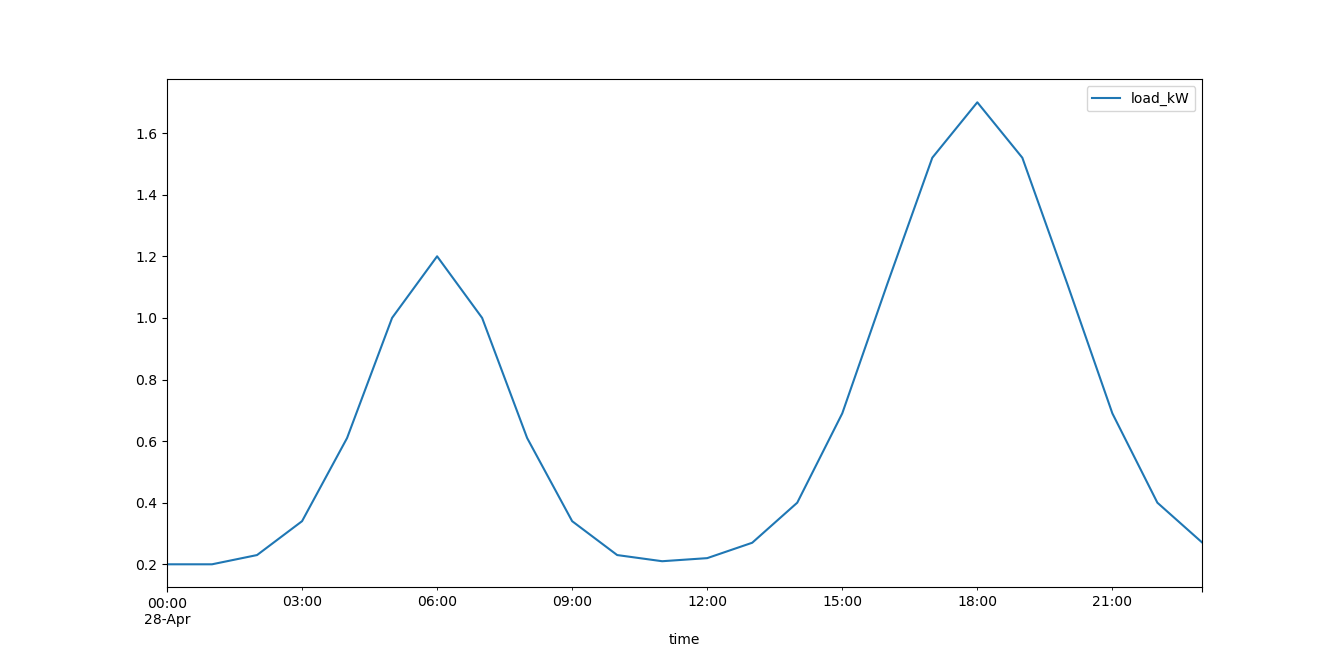
\includegraphics[width=0.7\textwidth]{../img/load.png}
		\caption{Curva original}\label{fig:load}
	\end{subfigure}
	\\ \vspace{0.1cm}
	\begin{subfigure}[b]{\textwidth}
		\centering
		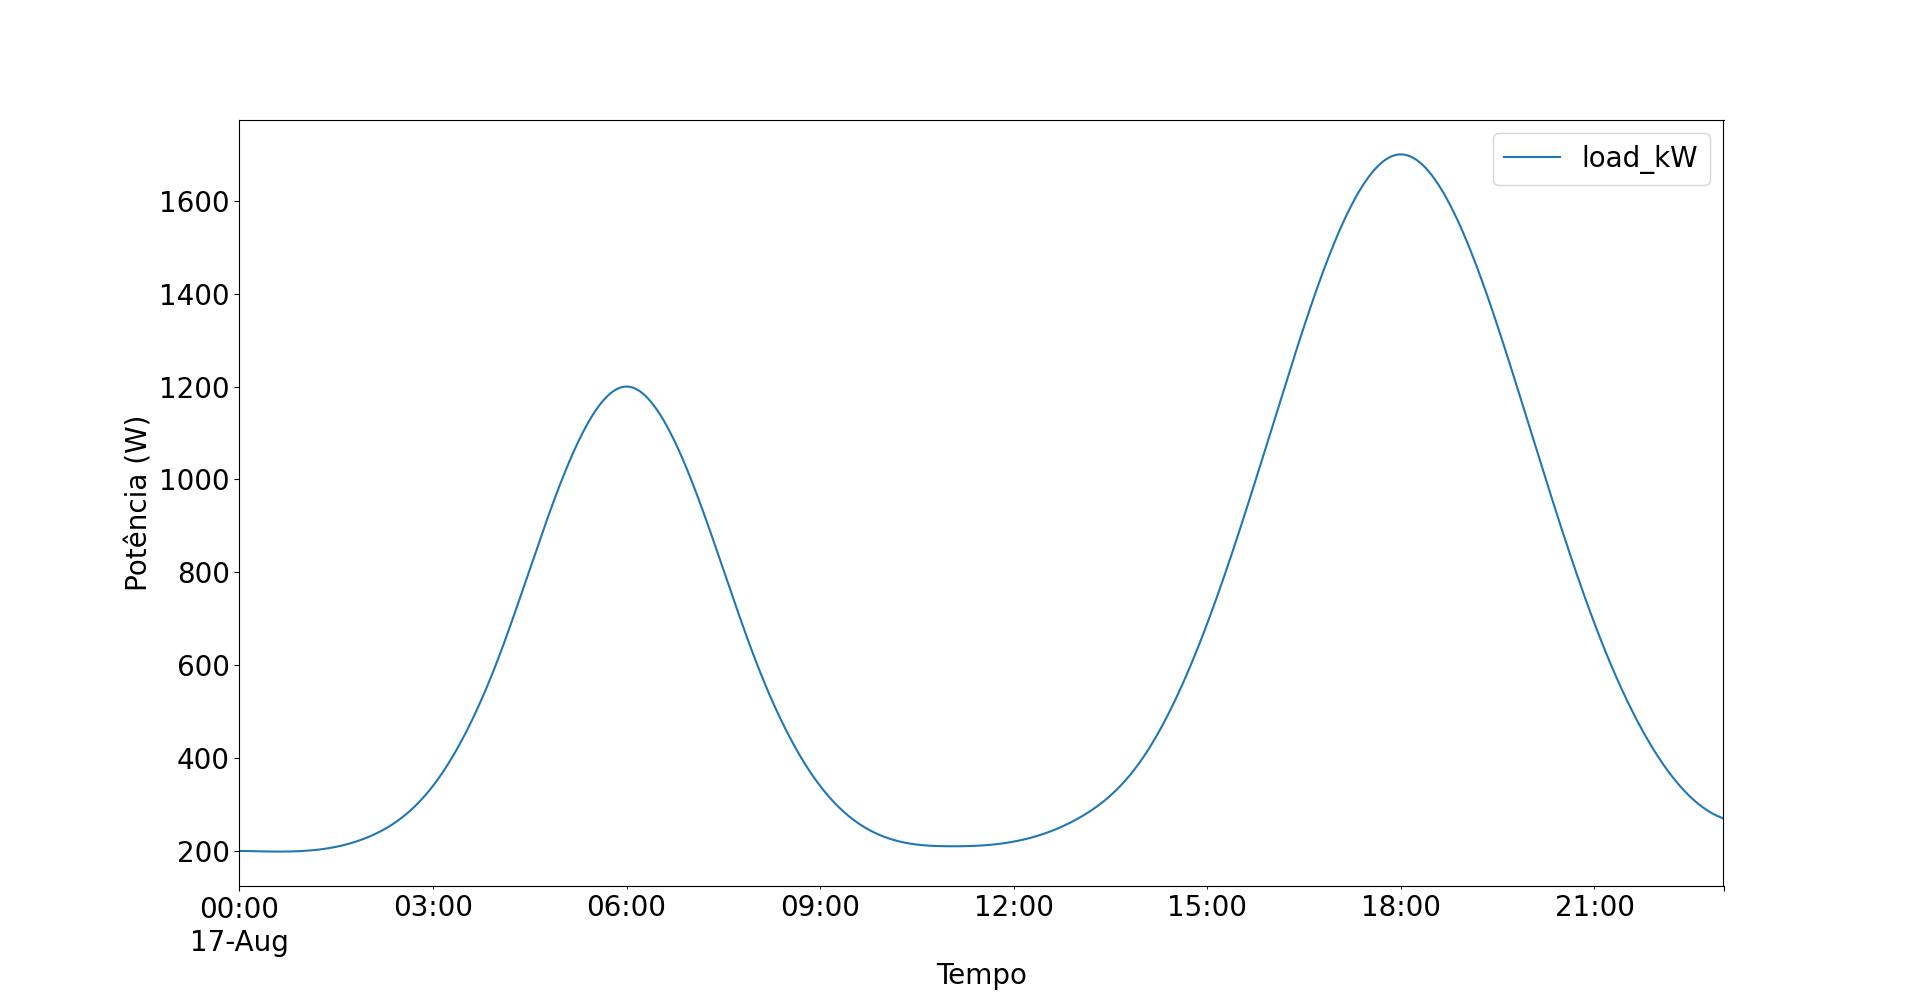
\includegraphics[width=0.7\textwidth]{../img/load_corr.png}
		\caption{Curva interpolada}\label{fig:load_corr}
	\end{subfigure}
	\caption{Perfil de carga de exemplo. Fonte: própria.}\label{fig:perfil}
\end{figure}


Os modelos a seguir foram considerados para cálculo de potência cada componente
do sistema.

\subsection{Solar}

A modelagem de um sistema fotovoltaico começa com o cálculo da irradiância
incidente no plano dos painéis. A irradiância $I_{T}$ é a soma da direta
$I_{b}$, difusa $I_{d}$ e a refletida $I_{r}$, proporcionais ao ângulo de
inclinação, de acordo com a Equação~\ref{eq:solar:it}.

\begin{equation}
  \label{eq:solar:it}   I_T = I_b R_b + I_d R_d + (I_b + I_d) R_r
\end{equation}

A potência dos painéis depende da área ocupada $A_{PV}$ e a eficiência $\eta$
dos módulos, de acordo com a Equação~\ref{eq:solar:p}.

\begin{align}
  \label{eq:solar:p}    P_{PV} &= I_T \eta A_{PV} \\
  \label{eq:solar:etam}    \eta_m &= \eta_r [1 - \beta (T_c - T_r)] \\
  \label{eq:solar:tc}   T_c &= T_a + \left(\frac{T_{\text{NOCT}}-20}{800}\right) I_T
\end{align}

O painel considerado foi o \emph{YGE 60 Cell Series 2}, com características na
Tabela~\ref{tbl:painel}.

% !TEX root = ../0_tcc.tex

\begin{table}[ht]
	\centering
	\caption{Painel YGE 60 Cell Series 2}\label{tbl:painel}
    \begin{tabular}{c r l}
		\hline
        Parâmetro    &   Valor & Unidade\\
		\hline
		\hline
        $\eta$       &  $19.6$ & $\cdot$  \\
        $\beta$      & $-0.30$ & T$^{-1}$ \\
        $A_{PV}$     &  $1.63$ & m$^2$    \\
		\hline
	\end{tabular}
\end{table}


\subsection{Eólica}

Para velocidade do vento medidas em uma altura diferente do cubo do aerogerador,
é preciso corrigir de acordo com a lei de cisalhamento vertical. As medições
mais próximas à superfície são menores devido ao à interação com o solo. A
medida que ascende-se, a velocidade torna-se logarítmicamente maior de acordo
com a Equação~\ref{eq:wind:pl}.

\begin{equation}
  \label{eq:wind:pl}  V_z = V_i \frac{Z}{Z_i}^x
\end{equation}

A curva de potência de um aerogerador é deduzida a partir de dados de campanhas
de medição do recurso eólico local.  Quando os dados disponíveis para o sistema
híbrido tem frequência diferente do que foi usado na campanha de medição, a
curva de potência original não é mais aplicável. Pode ser feita a correção da
curva introduzindo componentes estocásticas e determinísticas de acordo com o
modelo de Von-Kármán para rajadas de vento contínuas. Por motivos de
simplificação, foi considerado que a curva foi deduzida na mesma frequência
amostral da aplicação do sistema, dispensando correção.

A Turbina considerada foi o \emph{Bergey Excel-10}, com curva de potência na
Figura~\ref{fig:wind:power}. A curva também foi interpolada.

% !TEX root = ../0_tcc.tex

\begin{figure}[H]
	\centering
	\begin{subfigure}[b]{\textwidth}
		\centering
		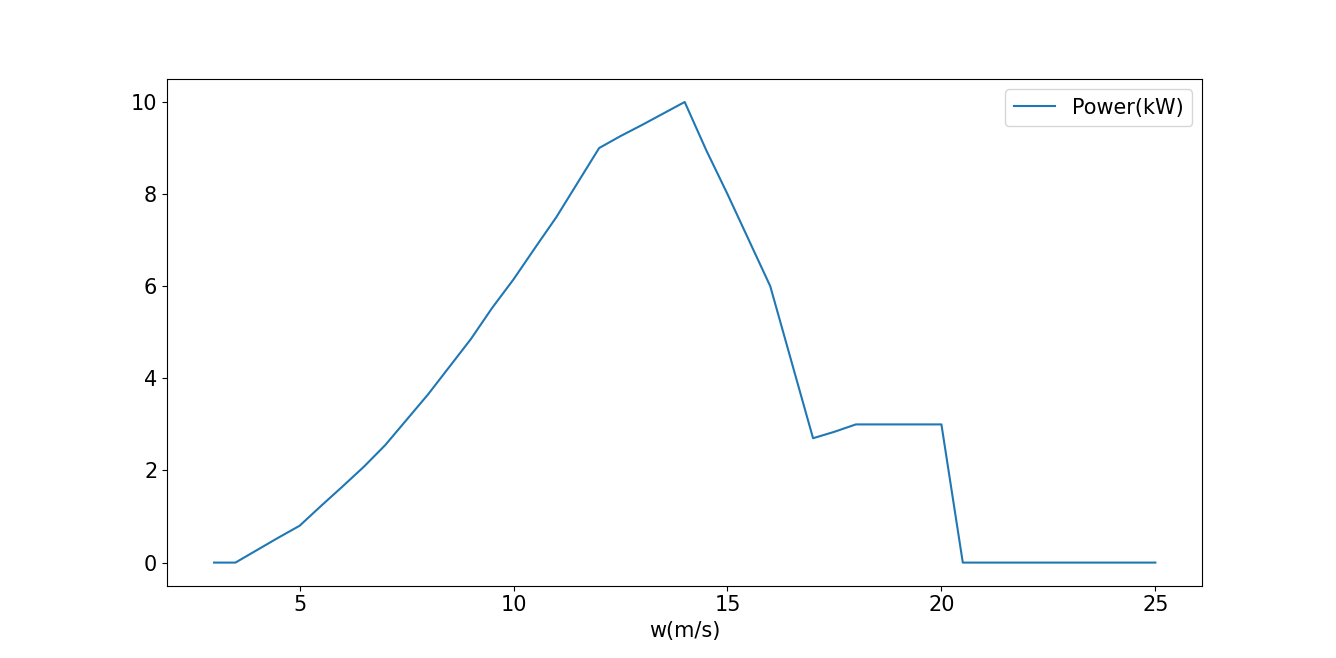
\includegraphics[width=0.8\textwidth]{../img/bergey.png}
		\caption{Curva original}\label{fig:bergey}
	\end{subfigure}
	\\ \vspace{0.5cm}
	\begin{subfigure}[b]{\textwidth}
		\centering
		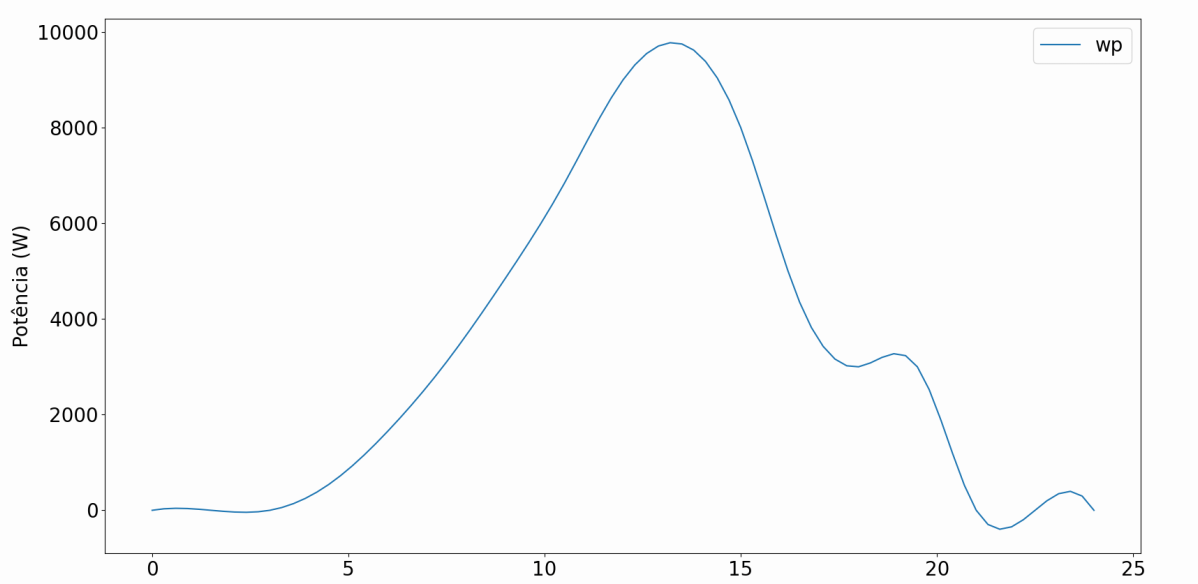
\includegraphics[width=0.8\textwidth]{../img/bergey_corr.png}
		\caption{Curva interpolada}\label{fig:bergey_corr}
	\end{subfigure}
	\caption{Curva de potência do aerogerador \emph{Bergey Excel-10}. Fonte: própria.}\label{fig:wind:power}
\end{figure}


\subsection{Diesel}

O grupo diesel ser modelado como uma função linear é uma suposição razoável de
acordo com resultados experimentais, como visto
em~\cite[cap.~6.1]{manwell2006hybrid2}. O coeficiente linear da função é o
consumo sem carga, com a máquina parada. A inclinação da reta é dada pela taxa
de consumo de combustível por unidade de potência de saída.  De acordo
com~\cite{Nema_2009}, para determinar a capacidade nominal do gerador diesel a
ser instalado, caso estiver diretamente conectado à carga, então o capacidade
nominal do gerador deve ser pelo menos igual à carga máxima.

\begin{align}
  \label{eq:diesel} F &= a + b P \\
  \nonumber a &= \text{consumo sem carga}\\
  \nonumber b &= \text{consumo por potência ($\ell$/kWh)}
\end{align}

O gerador diesel considerado foi o exemplo apresentado
em~\citeauthor{manwell2006hybrid2}, com características na
Tabela~\ref{tbl:diesel}.

% !TEX root = ../0_tcc.tex

\begin{table}[ht]
	\centering
	\caption{Gerador diesel}\label{tbl:diesel}
    \begin{tabular}{c r l}
		\hline
        Parâmetro        &  Valor & Unidade\\
		\hline
		\hline
        $P_{\text{nom}}$ &  $15$   & kW       \\
        $a$              &  $0$   & $\ell$/h   \\
        $b$              &  $1/3$   & {kWh}$^{-1}$    \\
		\hline
	\end{tabular}
\end{table}


\subsection{Bateria}

A capacidade do banco de baterias é dimensionado em função do tempo de
inatividade das outras fontes, referido como dias de autonomia.  Normalmente é
assumido 2 ou 3 dias de autonomia, ou seja: as baterias tem capacidade para
sustentar sozinhas o consumo por esse período.

As baterias são limitadas em um estado máximo e um mínimo de carga, não podendo
ultrapassá-los, como na Equação~\ref{eq:bat:lim}. O estado de carga pode ser
atualizado pelas equações~\ref{eq:bat:y1} e~\ref{eq:bat:y2} respeitando o modelo cinético de
baterias, \acrlong{kibam}.

\begin{equation}
  \label{eq:bat:lim}           \text{SOC}_{\text{min}} \leq \text{SOC}(t)   \leq \text{SOC}_{\text{max}}
\end{equation}

O \acrshort{kibam} consiste em admitir que um parte da capacidade está a
disposição para ser consumida imediadamente (\emph{available charge}) e outra
está confinada (\emph{bound charge}). Tal fato decorre da inércia da bateria em
transformar energia química em energia elétrica prontamente disponível para o
consumo.  O modelo restringe a mudança de carga de acordo com a
equação~\ref{eq:bat:y1} para a carga confinada e a equação~\ref{eq:bat:y2} para
carga disponível. Cada bateria possui um parâmetro $c$ que representa o
percentual de carga disponível e outo $k$ que mensura a velocidade de conversão
de energia.

\begin{align}
  \label{eq:bat:y1}    q_a(t+1) &= q_a r + \frac{(q_a k' c - i) (1 - r) - i c (k' t - 1 + r)}{k'} \\
  \label{eq:bat:y2}    q_b(t+1) &= q_b r + q_t (1 - c) (1 - r) - \frac{i (1 - c) k' t - 1 + r}{k'}
\end{align}

A bateria usada foi a \emph{Trojan Solar SPRE 12 225}, com especificações na
Tabela~\ref{tbl:bateria}.

% !TEX root = ../0_tcc.tex

\begin{table}[ht]
	\centering
	\caption{Bateria Trojan SPRE 12 225}\label{tbl:bateria}
    \begin{tabular}{c r l}
		\hline
		Parâmetro    &   Valor & Unidade\\
		\hline
		\hline
		$V$                         &  $12$    & V       \\
		$E_{\text{max}}$            &  $225$   & Ah      \\
		$\eta$                      &  $75\%$  & $\cdot$ \\
		$\text{SOC}_{\text{min}}$   &  $40\%$  & $\cdot$ \\
		$\text{SOC}_{\text{max}}$   &  $100\%$ & $\cdot$ \\
		\hline
	\end{tabular}
\end{table}


\subsection{Rede Neural}

A metodologia para previsão foi usar 36 instantes passados de tempo para prever
o comportamento meteorológico dos próximos 36 instantes.  Para isso, 36 redes
neurais foram treinadas, cada uma com o objetivo de prever um instante futuro
específico. A rede 1 prevê o instante $t+1$, a rede 2 prevê o instante $t+2$ e
assim em diante até a trigésima sexta. Todas recebem a mesma entrada, os 36
instantes passados, como ilustrado na Figura~\ref{tikz:nns}.  As séries
temporais usadas foram a de radiação solar e a velocidade do vento, cada uma com
suas respectivas previsões, totalizando 72 \acrshort{ann}s.

% !TEX root = ../0_tcc.tex

\begin{figure}[ht]
	\centering
		\begin{tikzpicture}
			\node[draw, rectangle]  at  (0,0)  (ts-36)
			{$t_{-35}, \dots, t_{-18}, \dots, t_{0} $};

			\node[draw, rectangle] at ([xshift=1cm]ts-36.east)   (ts1)   {$t_1$};
			\draw[->]  (ts-36.north) [bend left] to (ts1.north)  ;

			\node[draw, rectangle] at ([xshift=0.5cm]ts1.east)   (ts2)   {$t_2$};
			\draw[->]  (ts-36.north) [bend left] to (ts2.north)  ;

			\node[] at ([xshift=0.5cm]ts2.east)   (tsdot) {$\cdots$};

			\node[draw, rectangle] at ([xshift=0.5cm]tsdot.east) (ts18)  {$t_{18}$};
			\draw[->]  (ts-36.north) [bend left] to (ts18.north)  ;

			\node[] at ([xshift=0.5cm]ts18.east)   (tsdot2) {$\cdots$};

			\node[draw, rectangle] at ([xshift=0.5cm]tsdot2.east)  (ts36)  {$t_{36}$};
			\draw[->]  (ts-36.north) [bend left] to (ts36.north)  ;
		\end{tikzpicture}
	\caption{Esquema de várias redes para previsão individual de timesteps. Fonte: própria.}\label{tikz:nns}
\end{figure}


A arquitetura para todas redes foi a mesma, composta células \acrshort{rnn}
simples. O modelo foi feito utilizando o \emph{Keras}. A ferramenta é uma
\acrshort{api} do \emph{TensorFlow}, biblioteca de aprendizado de máquina
desenvolvida pelo \emph{Google}.  Para treinamento e teste da rede foi usado a
plataforma \emph{Google Colab} que permite computação em nuvem com
disponibilidade de \acrshort{gpu}. Outras arquiteturas foram avaliadas como a
\acrshort{lstm} mas, como obteve resultados semelhantes à \acrshort{rnn}, foi
escolhida a mais simples.

Os dados que entram na rede foram normalizados: subtraídos do menor valor e
divididos de pela diferença entre máximo e mínimo. O processo ilustrado pela
Equação~\ref{eq:minmax} tem objetivo de limitar os dados no intervalo de [0, 1].
Dessa forma, evita-se problemas de cálculo numérico como \emph{overflow} durante
o processo de treinamento e o gradiente descendente é capaz de convergir muito
mais rápido.

\begin{equation}
  \label{eq:minmax}   x_{i}' = \frac{x_{i} - x_{\text{min}}}{x_{\text{max}} - x_{\text{min}}}
\end{equation}

Além das células \acrshort{rnn}, também foi usado \emph{dropout}. A técnica
consiste em aleatoriamente desativar um percentual determinado de neurônios de
uma camada. Os neurônios desativados não passam informação à próxima camada.
Dessa forma, no processo de treinamento, a rede aprende a não depender de cada
neurônio individualmente, reduzindo a probabilidade de um nodo enviesar toda a
\acrshort{ann}. O sumário da rede é exibido na Tabela~\ref{tbl:model}.

% !TEX root = ../00_tcc.tex

\begin{table}[ht]
	\centering
	\caption{Modelo treinado}\label{tbl:model}
	\begin{subtable}{\textwidth}
		\centering
		\caption{Arquitetura}\label{tbl:model_arq}
		\begin{tabular}{c c c}
			\hline
			Camada   &   Shape de saída    &   Parâmetros\\
			\hline
			\hline
			SimpleRNN&   (None, 36, 64)   &   4224      \\
			Dropout  &   (None, 36, 64)   &   0         \\
			SimpleRNN&   (None, 32)       &   3104      \\
			Dropout  &   (None, 32)       &   0         \\
			Dense    &   (None, 1)        &   33        \\
			\hline
		\end{tabular}
	\end{subtable}
	\\ \vspace{1cm}
	\begin{subtable}{\textwidth}
		\centering
		\caption{Parâmetros}\label{tbl:model_param}
		\begin{tabular}{c c c}
			\hline
			Total de parâmetros & Parâmetros treináveis & Parâmetros não treináveis \\
			\hline
			\hline
			7,361        &    7,361         & 0 \\
			\hline
		\end{tabular}
	\end{subtable}
\end{table}


\subsection{Sistema Híbrido}

Foi considerado um sistema abastecido por 10 módulos fotovoltaicos, 1
aerogerador, 1 gerador diesel e banco de bateria com 1 dia de autonomia, como
mostrado na Tabela~\ref{tbl:sistema}.
Dessa forma, a tensão do barramento de corrente contínua ficou em 300 volts de
fotovoltaica mais 220 volts do aerogerador, totalizando 520.

% !TEX root = ../0_tcc.tex

\begin{table}[ht]
	\centering
	\caption{Sistema híbrido abordado}\label{tbl:sistema}
    \begin{tabular}{l l l}
		\hline
        Equipamento  &  Modelo     & Quantidade    \\
		\hline
		\hline
        Aerogerador          & Bergey Excel-10          & 1               \\
        Painel               & YGE 60 CELL Series 2     & 10              \\
		Gerador Diesel 15 kW &                          & 1               \\
		Baterias             & Trojan Solar SPRE 12 225 & 20              \\
		\hline
	\end{tabular}
\end{table}


Foi feita uma comparação considerando a \acrshort{lpsp} para as duas
estratégias: \acrshort{lf}.  O gerador diesel em
\acrshort{lf} entrará em operação caso a bateria não suprir o déficit,
acompanhando a carga líquida.  Em \acrshort{cc}, quando há déficit de energia, o
gerador diesel é ligado na máxima potência disponível que não gere excesso,
escoando a sobra para a bateria. Para manter a vida útil do gerador, tempos
mínimos de operação foram considerados.

% !TEX root = 00_tcc.tex
\clearpage

\section{Estudo de Caso}

Os dados avaliados possuíam considerável quantidade de \acrshort{nan}s, como
exposto na Tabela~\ref{tbl:nan}. Para evitar o comprometimento do modelo a ser
treinado, o período dos 3 primeiros meses de 2013 foram escolhidos para servir
de dado de entrada.  O período for composto dos 3 primeiros meses do ano. Os
dados foram separados em grupos: treinamento com 75\% e teste com 25\% do total.
Dessa forma, foram 2 meses para treinamento do modelo e 1 para teste.

% !TEX root = ../0_tcc.tex

\begin{table}[ht]
	\centering
	\caption{Quantidade de \acrshort{nan}s}\label{tbl:nan}
	\begin{tabular}{lrr}
		\hline
		Data & WS\_10m &     GHI \\
		\hline
		\hline
		2006 &       0 &       0 \\
		2007 &   58185 &   58185 \\
		2008 &  137714 &  137714 \\
		2009 &   26791 &   26791 \\
		2010 &    5651 &    5651 \\
		2011 &    3120 &    3120 \\
		2012 &   38798 &   38798 \\
		2013 &    5520 &   11269 \\
		2014 &       3 &    2106 \\
		2015 &   10278 &   39468 \\
		2016 &   13380 &   21841 \\
		2017 &  126826 &  126826 \\
		\hline
	\end{tabular}
\end{table}


A velocidade do vento no local foi insuficiente para manter a operação da
aerogerador por longos períodos, devido a sua velocidade de \emph{cut-in}. O
histograma da Figura~\ref{fig:hist} mostra a frequência da velocidade corrigida
pela Equação~\ref{eq:wind:pl} para uma altura de 35 metros. Percebe-se que a
maioria encontra-se ao redor de 4 $m/s$, próximo ao começo de operação.

\begin{figure}[ht]
	\centering
	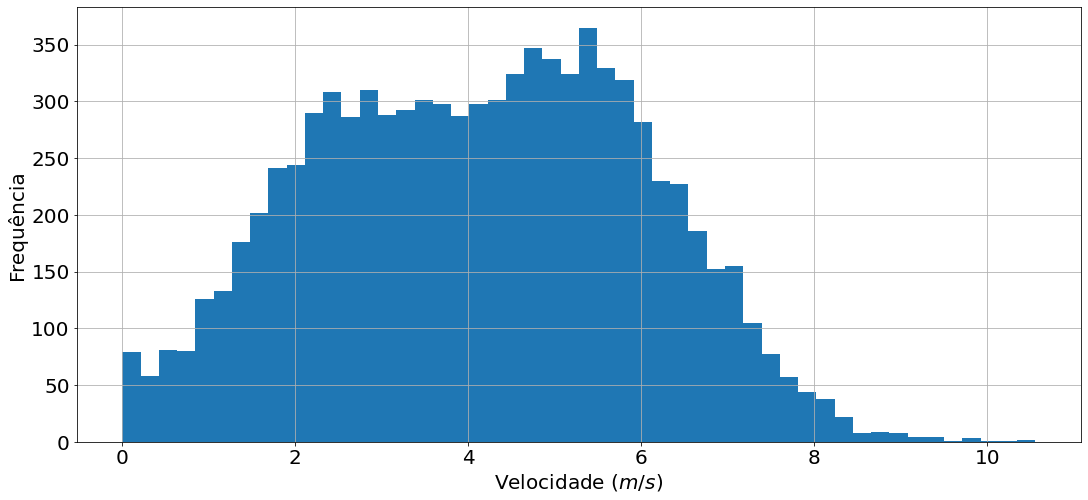
\includegraphics[width=0.8\textwidth]{../img/wind_hist.png}
	\caption{Histograma da velocidade do vento}\label{fig:hist}
\end{figure}

\subsection{Resultados}

O treinamento das redes atingiu baixos valores de \acrshort{rmse}, permanecendo
na segunda casa decimal, em parte por causa da normalização da
Equação~\ref{eq:minmax}. Ficou perceptível que a medida em que tenta-se realizar
predições de mais longo prazo, o desempenho diminui, como exposto na
Figura~\ref{fig:rmse}. Na figura, a linha laranja, com legenda de
\acrshort{ghi}\footnote{\acrlong{ghi}}, representa as redes de previsão solar. A
linha azul, \acrshort{ws10m}\footnote{\acrlong{ws10m}}, representa as redes de
previsão eólica.

\begin{figure}[ht]
	\centering
	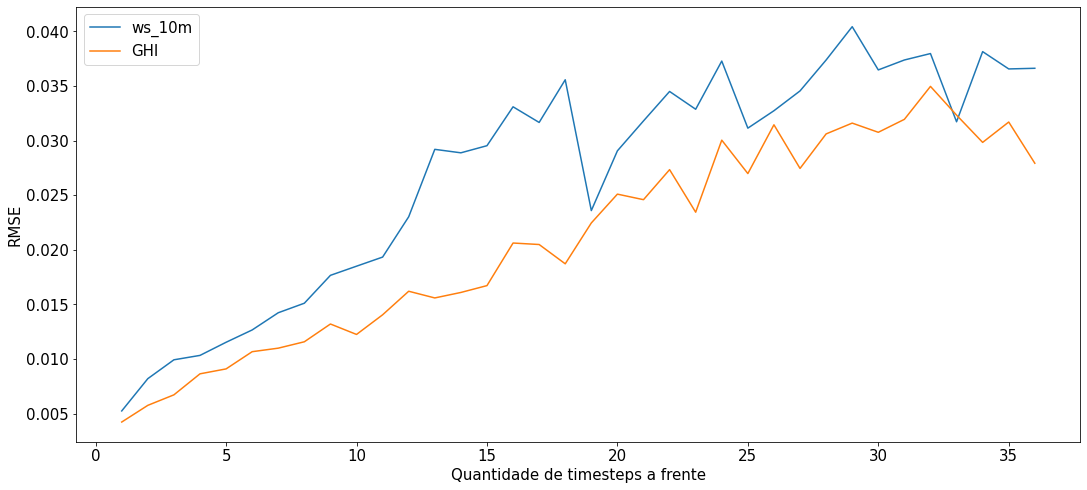
\includegraphics[width=0.8\textwidth]{../img/rmse_last3m.png}
	\caption{\acrshort{rmse} final de cada rede}\label{fig:rmse}
\end{figure}

As previsões da rede eólica inicialmente seguiram os dados mas nas últimas pode
se ver que o comportamento é descaracterizado. O algoritmo aprendeu a prever a
média de forma a reduzir a função custo, como visto na
Figura~\ref{fig:wind:pred}.  A previsão solar teve melhor desempenho, com mais
fidelidade aos dados. Ainda sim, os períodos noturnos provocaram platôs de
inércia, vistos na Figura~\ref{fig:solar:pred18} e~\ref{fig:solar:pred-1}.

% !TEX root = ../0_tcc.tex

\begin{figure}[H]
	\centering
	\begin{subfigure}{\textwidth}
		\centering
		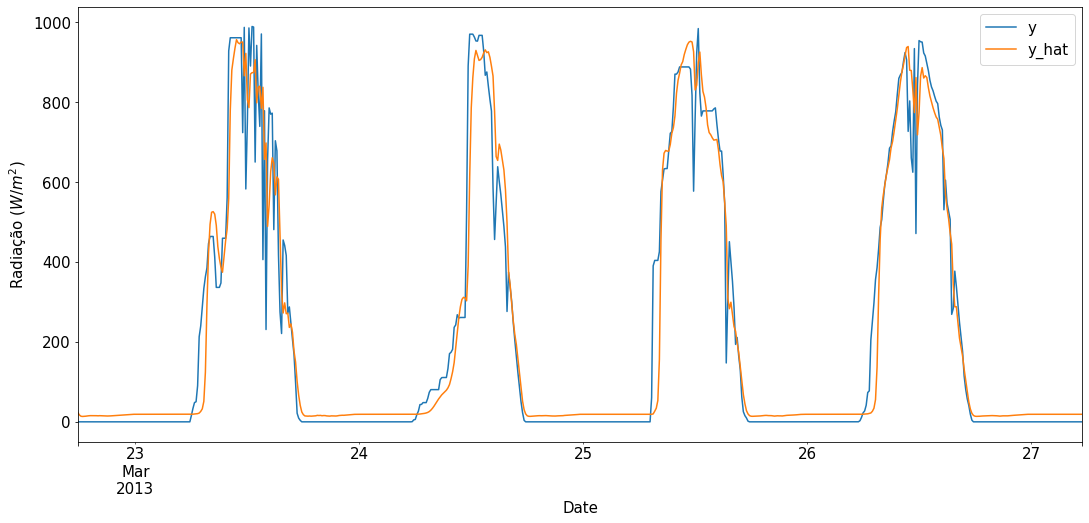
\includegraphics[width=0.7\textwidth]{../img/solar_pred_3m_0.png}
		\caption{Previsão realizada pela primeira rede}\label{fig:solar:pred1}
	\end{subfigure}
	\\ \vspace{1cm}
	\begin{subfigure}{\textwidth}
		\centering
		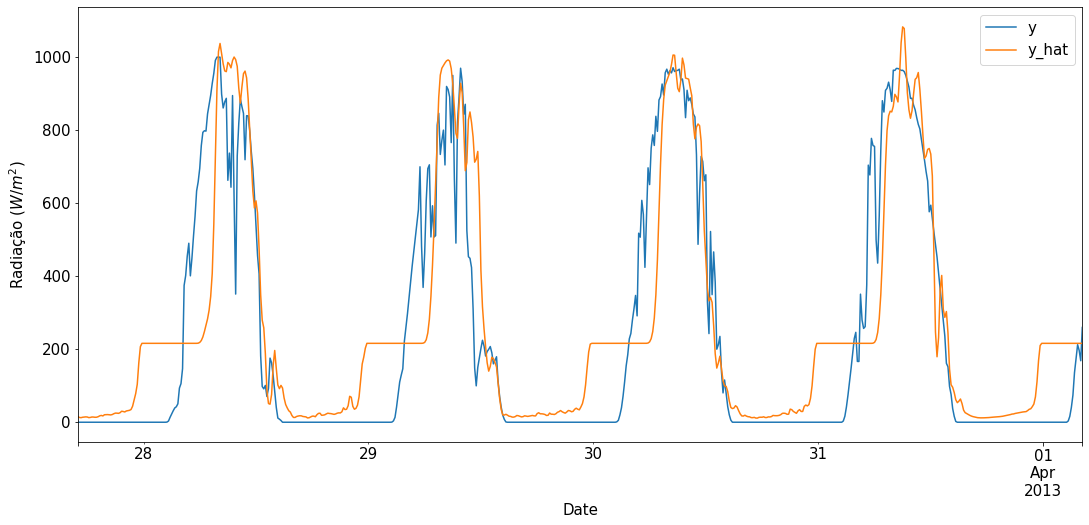
\includegraphics[width=0.7\textwidth]{../img/solar_pred_3m_18.png}
		\caption{Previsão realizada pela décima oitava rede}\label{fig:solar:pred18}
	\end{subfigure}
	\\ \vspace{1cm}
	\begin{subfigure}{\textwidth}
		\centering
		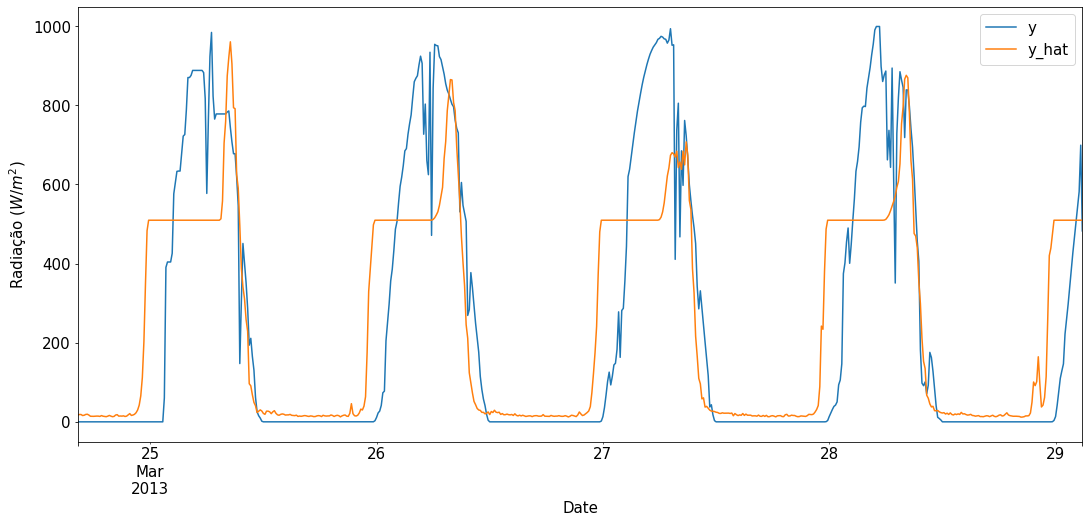
\includegraphics[width=0.7\textwidth]{../img/solar_pred_3m_-1.png}
		\caption{Previsão realizada pela última rede}\label{fig:solar:pred-1}
	\end{subfigure}
	\caption{Previsão de irradiação nos dados de teste}\label{fig:solar:pred}
\end{figure}


% !TEX root = ../00_tcc.tex

\begin{figure}[H]
	\centering
	\begin{subfigure}{\textwidth}
		\centering
		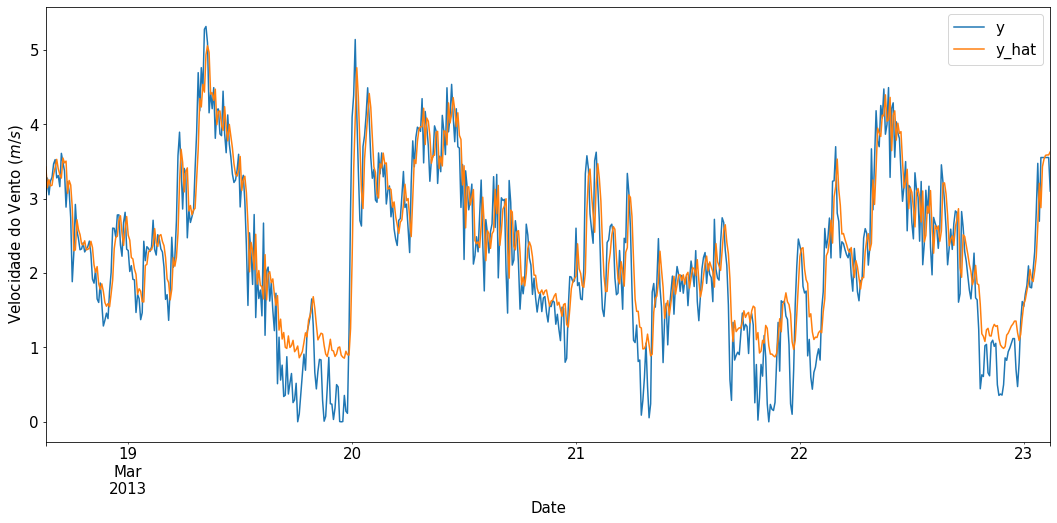
\includegraphics[width=0.7\textwidth]{../img/wind_pred_3m_0.png}
		\caption{Previsão realizada pela primeira rede}\label{fig:wind:pred1}
	\end{subfigure}
	\\ \vspace{1cm}
	\begin{subfigure}{\textwidth}
		\centering
		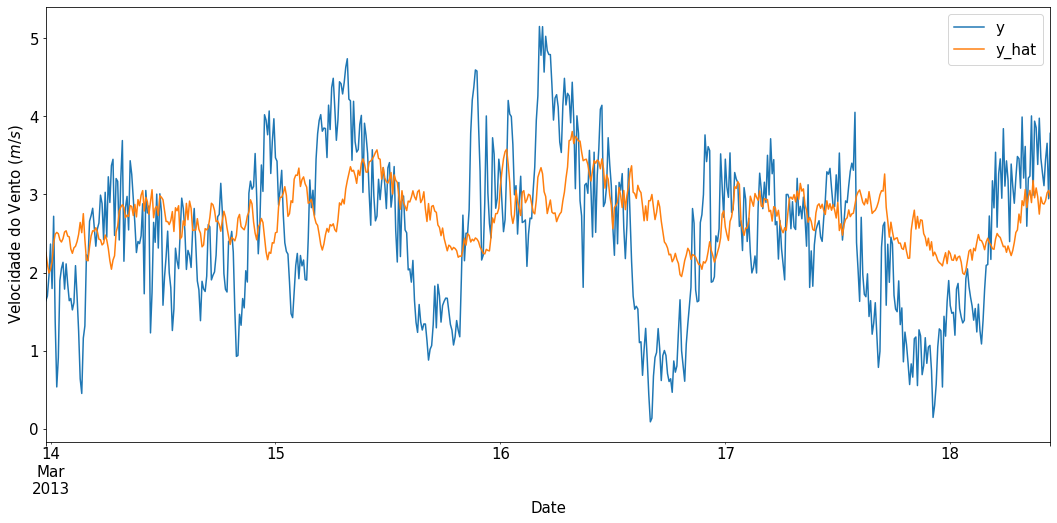
\includegraphics[width=0.7\textwidth]{../img/wind_pred_3m_18.png}
		\caption{Previsão realizada pela décima oitava rede}\label{fig:wind:pred18}
	\end{subfigure}
	\\ \vspace{1cm}
	\begin{subfigure}{\textwidth}
		\centering
		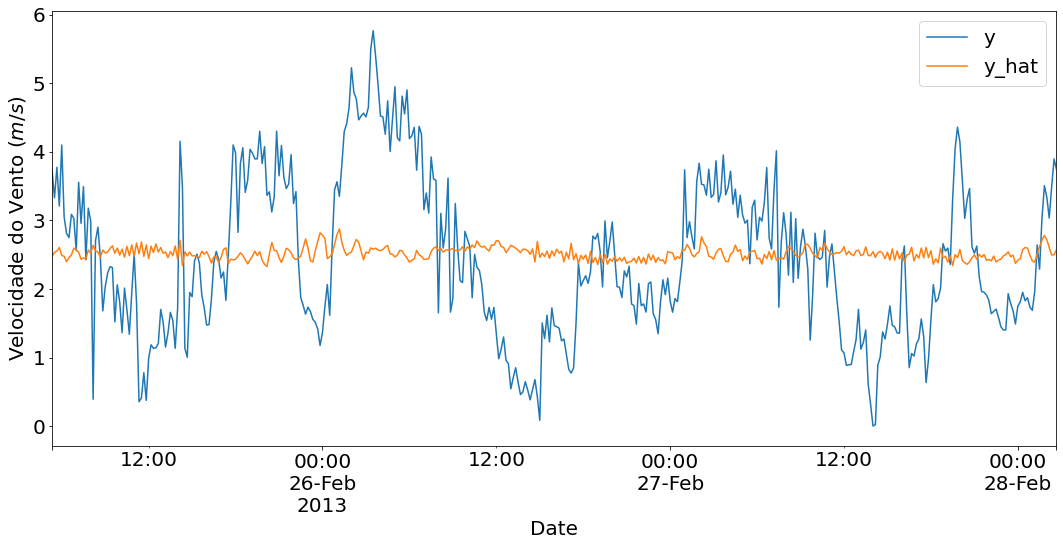
\includegraphics[width=0.7\textwidth]{../img/wind_pred_3m_-1.png}
		\caption{Previsão realizada pela última rede}\label{fig:wind:pred-1}
	\end{subfigure}
	\caption{Previsão de velocidade do vento nos dados de teste}\label{fig:wind:pred}
\end{figure}


Quando aplicadas em conjunto com uma previsão de cada rede, nas
figuras~\ref{fig:solar:comp} e~\ref{fig:wind:comp},  o resultado aparentou
ser satisfatório.

% !TEX root = ../0_tcc.tex

\begin{figure}[H]
	\centering
	\begin{subfigure}{\textwidth}
		\centering
		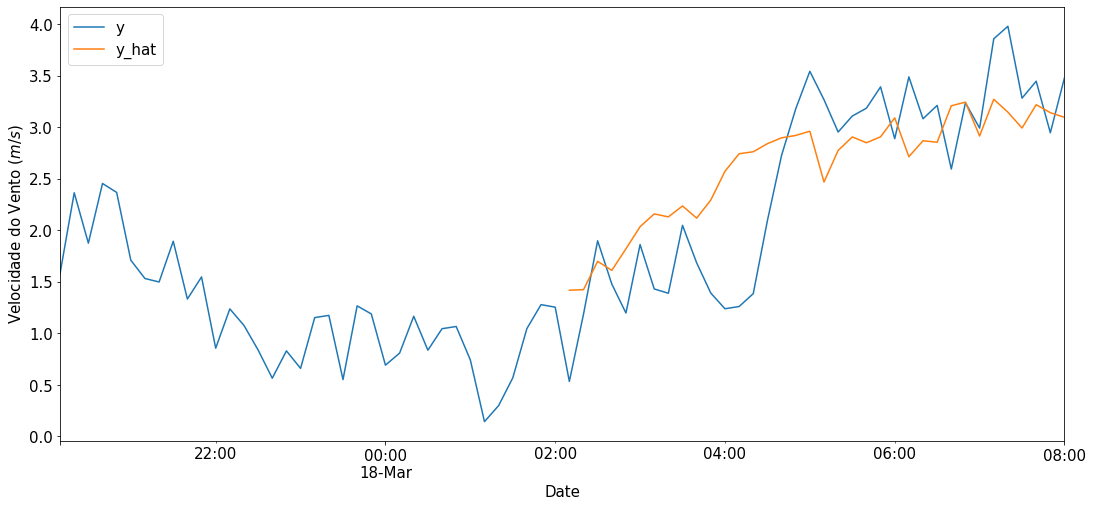
\includegraphics[width=0.8\textwidth]{../img/wind_comp.png}
		\caption{Previsão eólica}\label{fig:wind:comp}
	\end{subfigure}
	\\ \vspace{1cm}
	\begin{subfigure}{\textwidth}
		\centering
		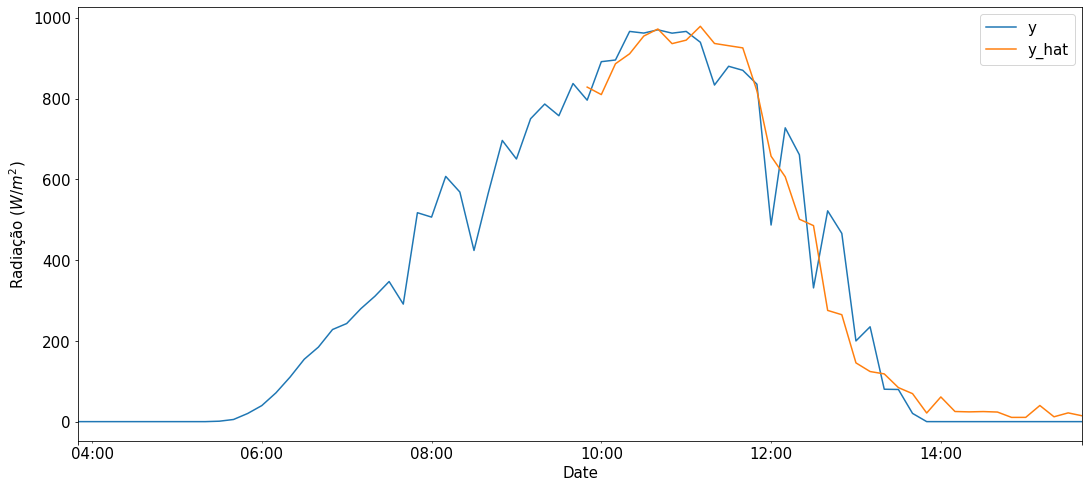
\includegraphics[width=0.8\textwidth]{../img/solar_comp.png}
		\caption{Previsão solar}\label{fig:solar:comp}
	\end{subfigure}
	\caption{Previsão final comparada aos dados reais}\label{fig:comp}
\end{figure}


Com apenas fontes renováveis, o sistema apresentou alto índice de \acrlong{lpsp},
com déficit em 46\% dos instantes de tempo. No cenário de uma única
estratégia de controle para o sistema, a \acrshort{lpsp} caiu consideravelmente.
Diante dessas condições, quando aplicada apenas a estratégia de \acrshort{cc}, é
obtido 5,94\% de \acrshort{lpsp}, já no caso de \acrshort{lf} o percentual é de
7,69\%.

Para mensurar a aplicabilidade de estratégias preditivas, foram feitas previsões
da radiação solar e velocidade do vento para todos intervalos. Em posse das
previsões, métricas foram calculadas em todos os instantes da série temporal.  O
primeiro instante considera a janela de $t$ até $t+36$, o segundo considera
$t+1$ até $t+37$ e assim por diante.  Em cada uma dessas janelas, 4 cenários de
\acrlong{lpsp} foram avaliados: apenas com \acrshort{lf} para dados reais,
apenas com \acrshort{cc} para dados reais e o mesmo para as previsões.  A melhor
estratégia dos dados reais foi comparada com a melhor estratégia prevista pelo
modelo. Caso os resultados fossem iguais, a previsão foi correta.

Inicialmente, o diesel poderia arrancar e parar em qualquer instante, por isso o
comportamento de \acrshort{cc} e \acrshort{lf} foi praticamente o mesmo. Foi
introduzida uma limitação ao grupo diesel de mínimo tempo de execução, uma vez
iniciado. A limitação é comum em máquinas térmicas, com vista a preservar a vida
útil do equipamento. Foram avaliados diferentes valores para o mínimo tempo de
execução.
O estado de carga da bateria exibido na Figura~\ref{fig:soc} ilustra
a diferença de comportamento. Devido à \acrshort{cc} arrancar sempre com maior
potência disponível, a estratégia teve melhor \acrshort{lpsp}.

% !TEX root = ../00_tcc.tex

\begin{figure}[H]
	\centering
	\begin{subfigure}{\textwidth}
		\centering
		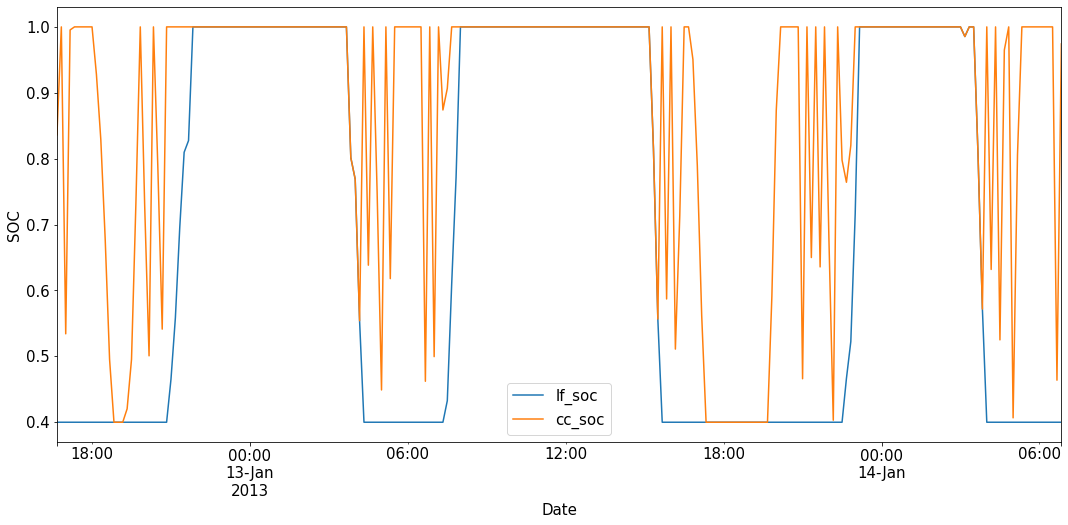
\includegraphics[width=0.7\textwidth]{../img/soc.png}
		\caption{Sem tempo mínimo de funcionamento}\label{fig:soc0}
	\end{subfigure}
	\\ \vspace{1cm}
	\begin{subfigure}{\textwidth}
		\centering
		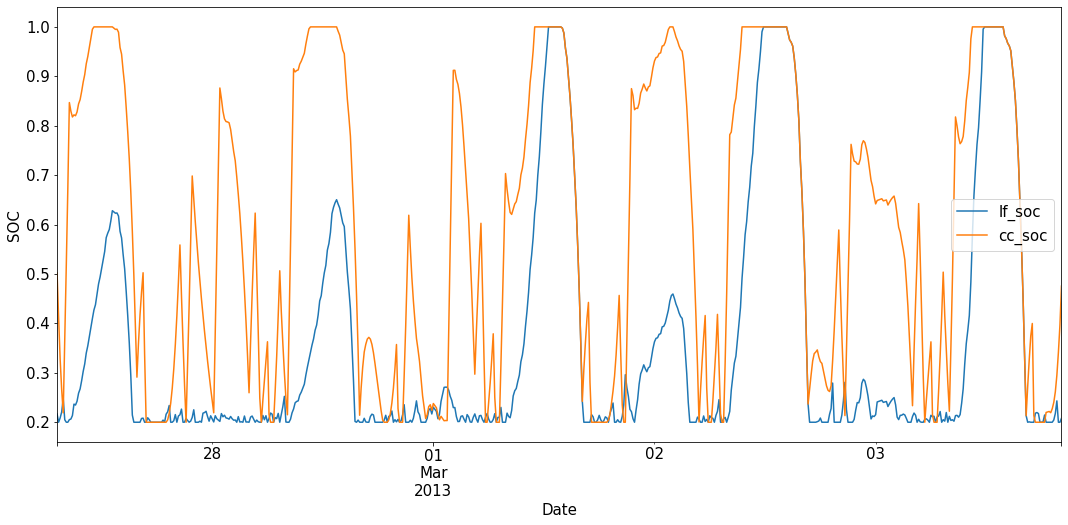
\includegraphics[width=0.7\textwidth]{../img/soc_3.png}
		\caption{Mínima excecução de 3 intervalos}\label{fig:soc3}
	\end{subfigure}
	\\ \vspace{1cm}
	\begin{subfigure}{\textwidth}
		\centering
		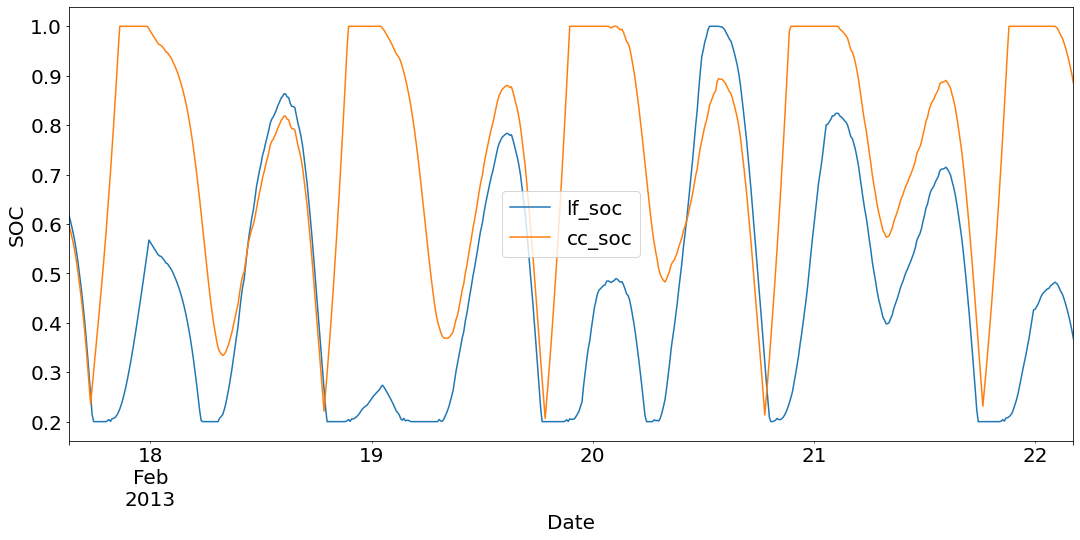
\includegraphics[width=0.7\textwidth]{../img/soc_6.png}
		\caption{Mínima excecução de 6 intervalos}\label{fig:soc6}
	\end{subfigure}
	\caption{Comparação da oscilação do \acrshort{soc}}\label{fig:soc}
\end{figure}


Os resultados para um mínimo tempo do diesel de 6 intervalos foram traçados em
uma matriz de confusão, visto na Figura~\ref{fig:confusion}. As previsões
apresentaram cerca de 75\% de acurácia, tendo previsto
corretamente~\acrshort{lf} como maior \acrshort{lpsp}.

\begin{figure}[H]
	\centering
	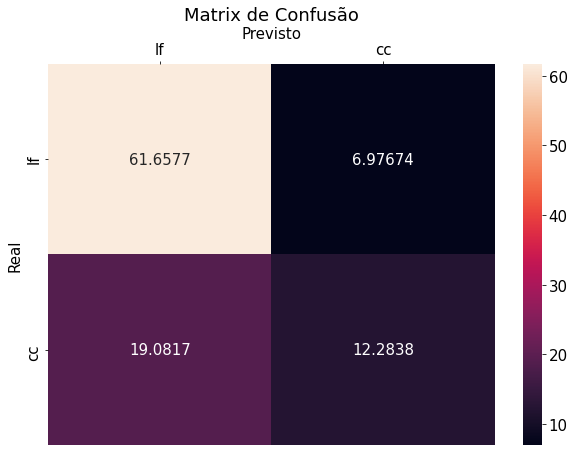
\includegraphics[width=0.6\textwidth]{../img/hm_cc.png}
	\caption{Resultados para previsão}\label{fig:confusion}
\end{figure}

O controle preditivo conseguiu resultados intermediários como exposto na
Tabela~\ref{tbl:comp}.  O comportamento de \acrshort{lpsp} está de acordo com o
estudo de~\cite{das2019performance}, que avalia diferentes estratégias de
controle. No trabalho, é concluído que, no cenário em questão, a maior diferença
entre \acrshort{lf} e \acrshort{cc} é a fração renovável de cada uma e,
consequentemente, o consumo de diesel.

% !TEX root = ../0_tcc.tex

\begin{table}[ht]
	\centering
	\caption{Comparativo de estratégias}\label{tbl:comp}
	\begin{tabular}{lrrr}
		\hline
		                & \acrshort{lf}   & \acrshort{cc} &  \acrshort{lf} e \acrshort{cc} \\
		\hline
		\hline
		\acrshort{lpsp} &  5.94\%         &  7.69\%       &  6.87\%                        \\
		\hline
	\end{tabular}
\end{table}


O \emph{Google Colab} mostrou-se útil para construção e treinamento de modelos
em uma máquina remota.  O uso da ferramenta gratuita pode facilitar
investimentos com pouca disponibilidade de recursos computacionais.As redes
neurais apresentaram baixo \acrshort{rmse}, entretanto previsões de mais longo
prazo mostraram comportamentos errôneos: a solar não previu os picos diários,
compensando em previsões negativas ao fim do dia e a rede eólica seguiu a
tendência mas não acompanhou a amplitude do sinal.  O sistema abastecido apenas
por fontes renováveis apresentou alta probabilidade de perda de carga. Quando
aplicadas as estratégias, tanto \acrshort{lf} quanto \acrshort{cc}, a
\acrshort{lpsp} diminuiu consideravelmente.  Entretanto, o comportamento
preditivo das estratégias foi similar devido à liberdade de arrancar e parar o
gerador diesel a qualquer momento.  Quando introduzido limitações de tempo
mínimo de operação, \acrshort{cc} se tornou a estratégia mais confiável por
causa de sua potência de arranque mais alta.

% !TEX root = 0_tcc.tex
\clearpage

\section{Conclusão e Perspectivas}

Como visto em, o processo de aplicação de um sistema híbrido é uma problemática
com diversos fatores que a influenciam, desde a idealização até operação.  As
fases de configuração, dimensionamento e operação passam todas por processos de
otimização, cada uma com particularidades.  As métricas abordadas auxiliaram em
decisões de desenho melhores.

A utilização da mesma arquitetura para todas \acrshort{ann} pode ter sido uma
das causas, visto que os fenômenos meteorológicos tem frequências diferentes,
como início e fim do dia ou estações do ano. Melhorias podem ser feitas através
da decomposição dos sinais, como no estudo de~\cite{Liu_2018}, citado
anteriormente.  Para as redes da irradiação solar, em estudos futuros é possível
conseguir melhores resultados realizando treinamento em dados apenas do período
diurno. Para determinar momentos em que há sol, o ângulo azimutal pode ser
indicador, considerando limites de nascer e pôr do sol. Uma função custo
diferente, como a correlação, para o treinamento poderia minimizar a diferença
de amplitude de sinal causada com a \acrshort{rmse}.

Os resultados expuseram que,  quando aplicada em contextos mais simples, as
estratégia se assemelham. A aplicação pode ser estudada com maior granularidade
nos critérios para uma avaliação mais diversa.

% !TEX root = 00_tcc.tex
\clearpage
\printbibliography[heading=bibintoc]

% !TEX root = 0_tcc.tex
\clearpage{}
\small \singlespacing{}
\begin{appendices}

\section{Rede Neural}

\lstinputlisting[
	language=Python,
	breaklines,
	numbers=left
]{../code/nn.py}

\clearpage{}

\section{Sistema Híbrido}

\lstinputlisting[
	language=Python,
	breaklines,
	numbers=left
]{../code/hres.py}

\clearpage{}

\section{Estratégias}

\lstinputlisting[
	language=Python,
	breaklines,
	numbers=left
]{../code/dispatch.py}

\end{appendices}


\end{document}
